\newpage
\begin{figure}
    \begin{subfigure}{.5\textwidth}
        \centering
        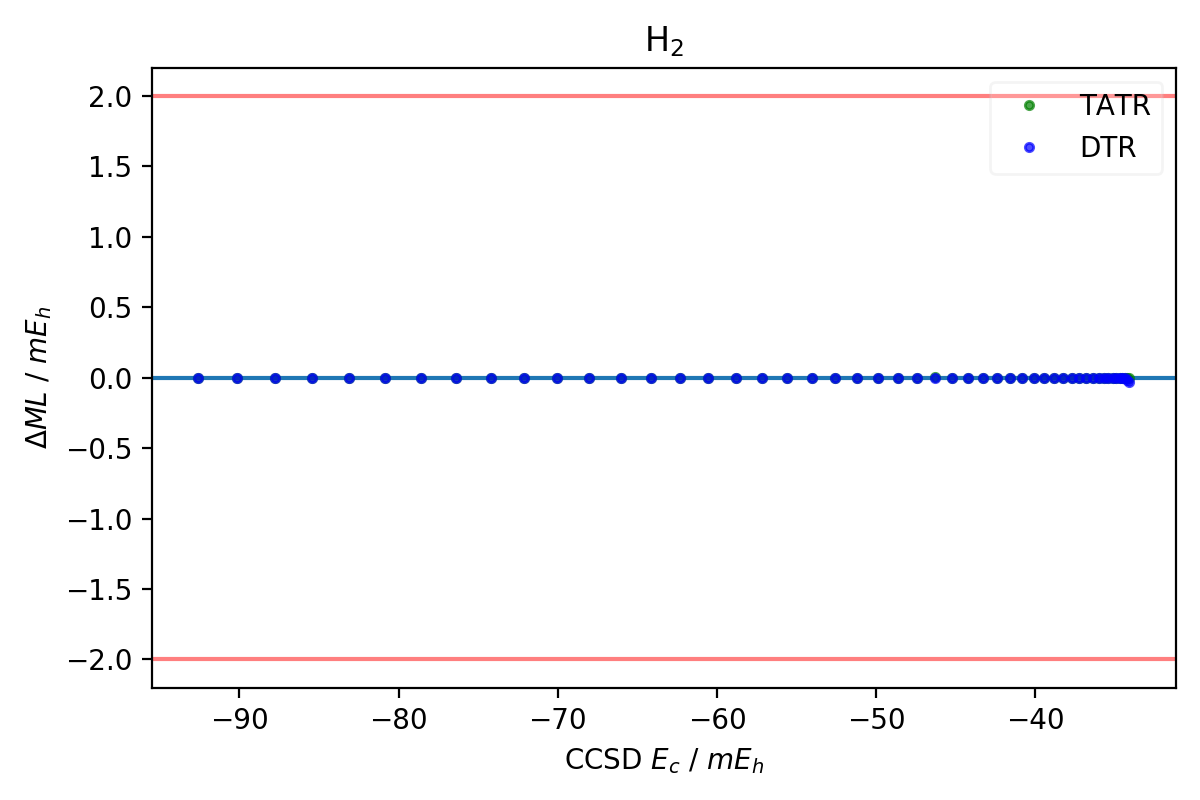
\includegraphics[scale=.55]{p2/figures/si/H2_e.png}
        \caption{}
        \label{fig:H2}
    \end{subfigure}%
    \begin{subfigure}{.5\textwidth}
        \centering
        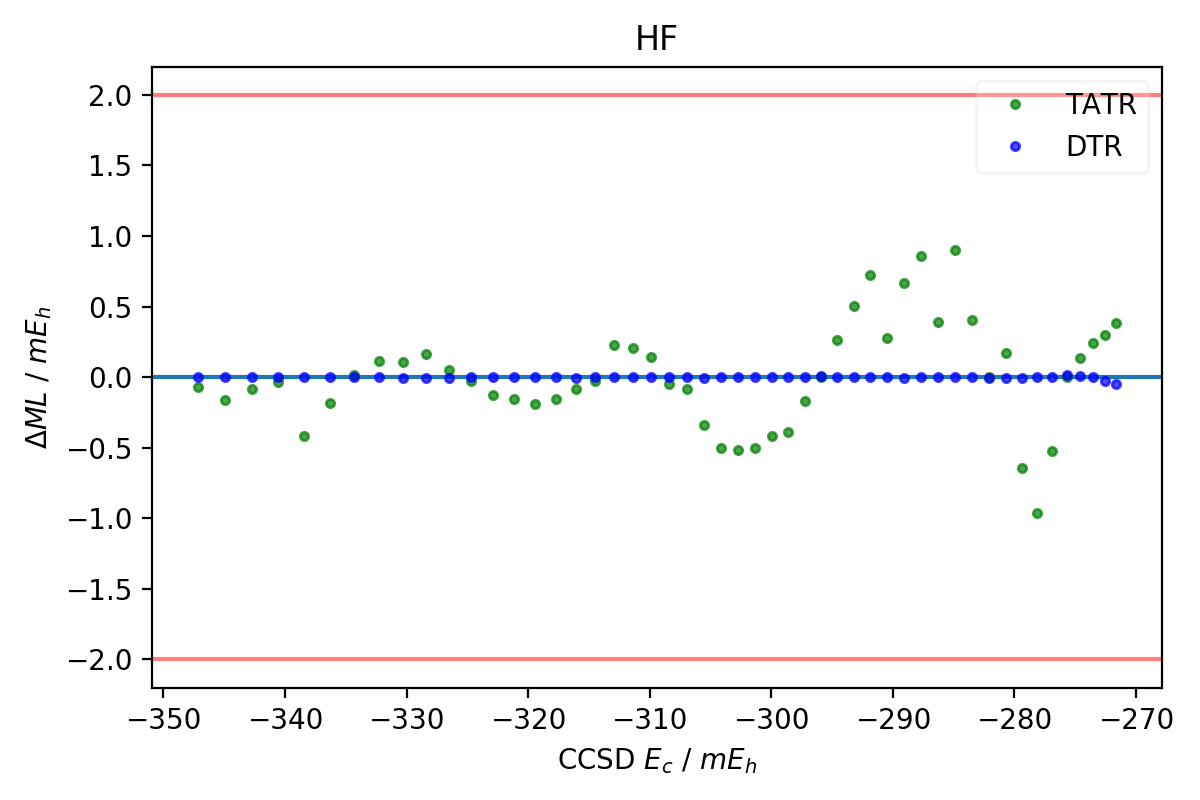
\includegraphics[scale=.55]{p2/figures/si/HF_e.png}
        \caption{}
        \label{fig:HF}
    \end{subfigure}
    \begin{subfigure}{.5\textwidth}
        \centering
        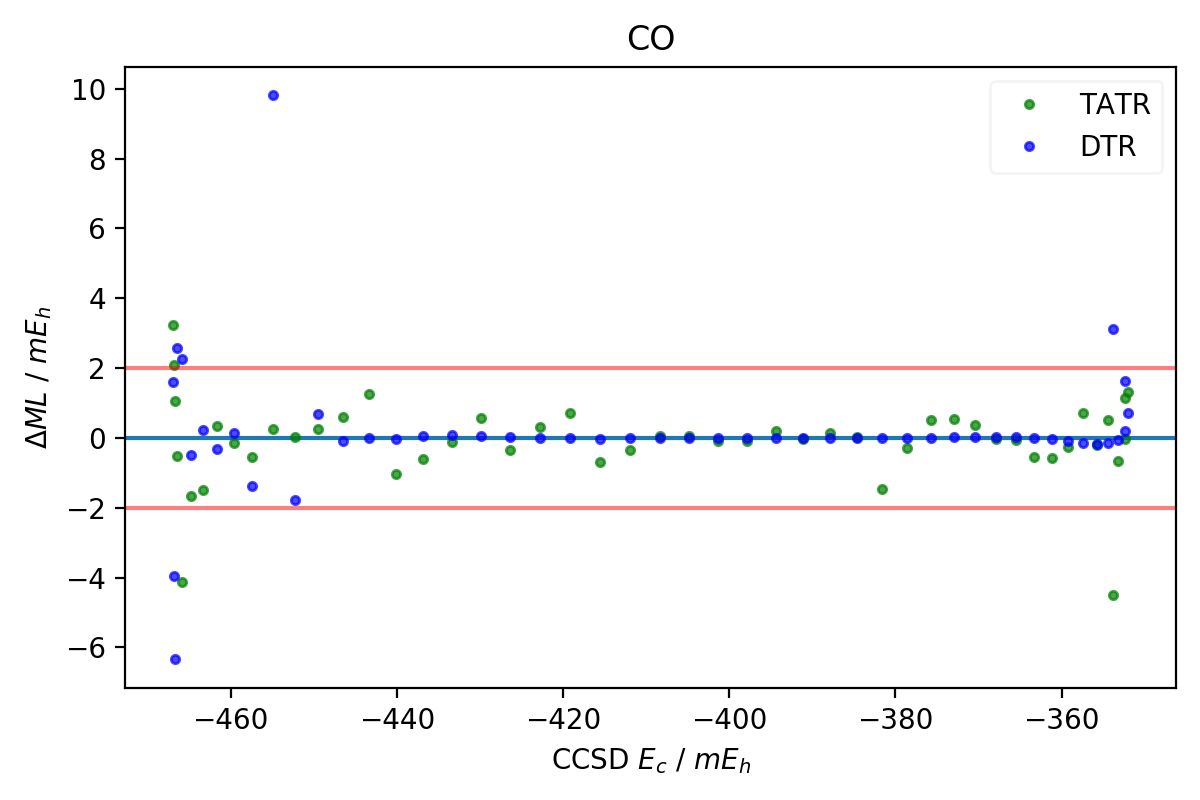
\includegraphics[scale=.55]{p2/figures/si/CO_e.png}
        \caption{}
        \label{fig:CO}
    \end{subfigure}%
    \begin{subfigure}{.5\textwidth}
        \centering
        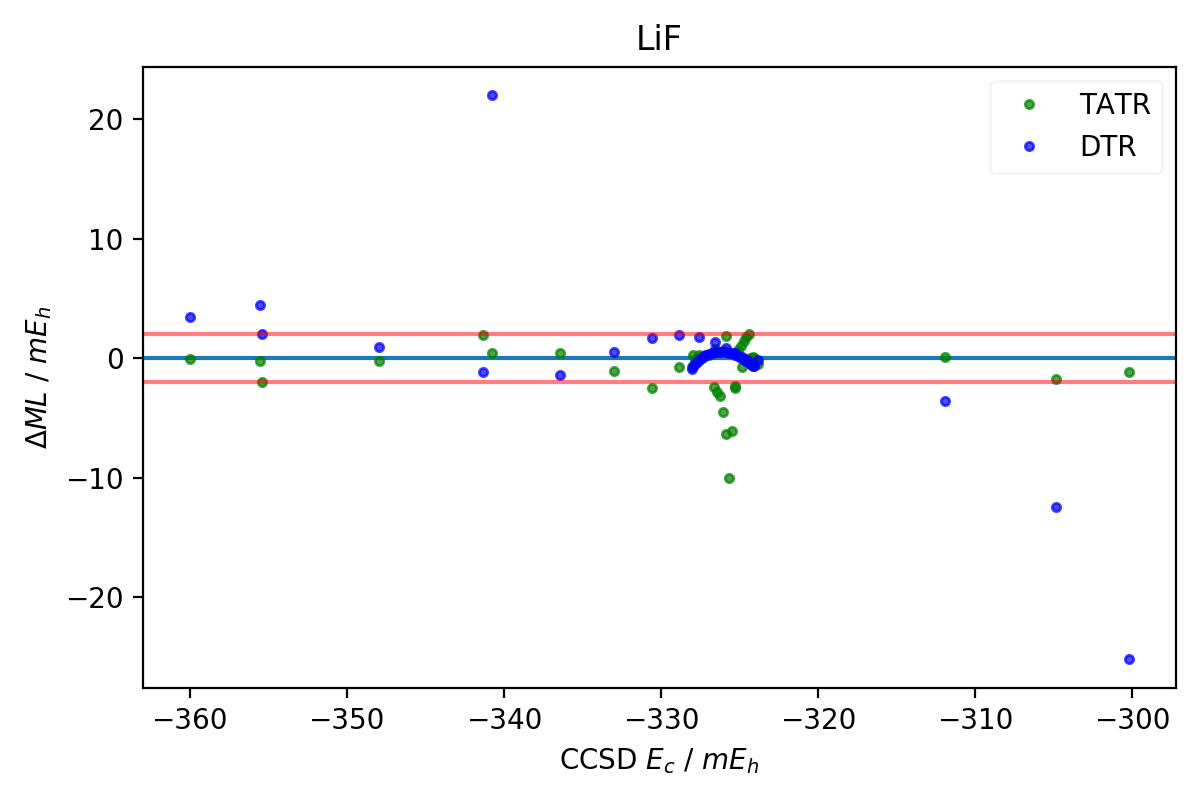
\includegraphics[scale=.55]{p2/figures/si/LiF_e.png}
        \caption{}
        \label{fig:LiF}
    \end{subfigure}
    \begin{subfigure}{.5\textwidth}
        \centering
        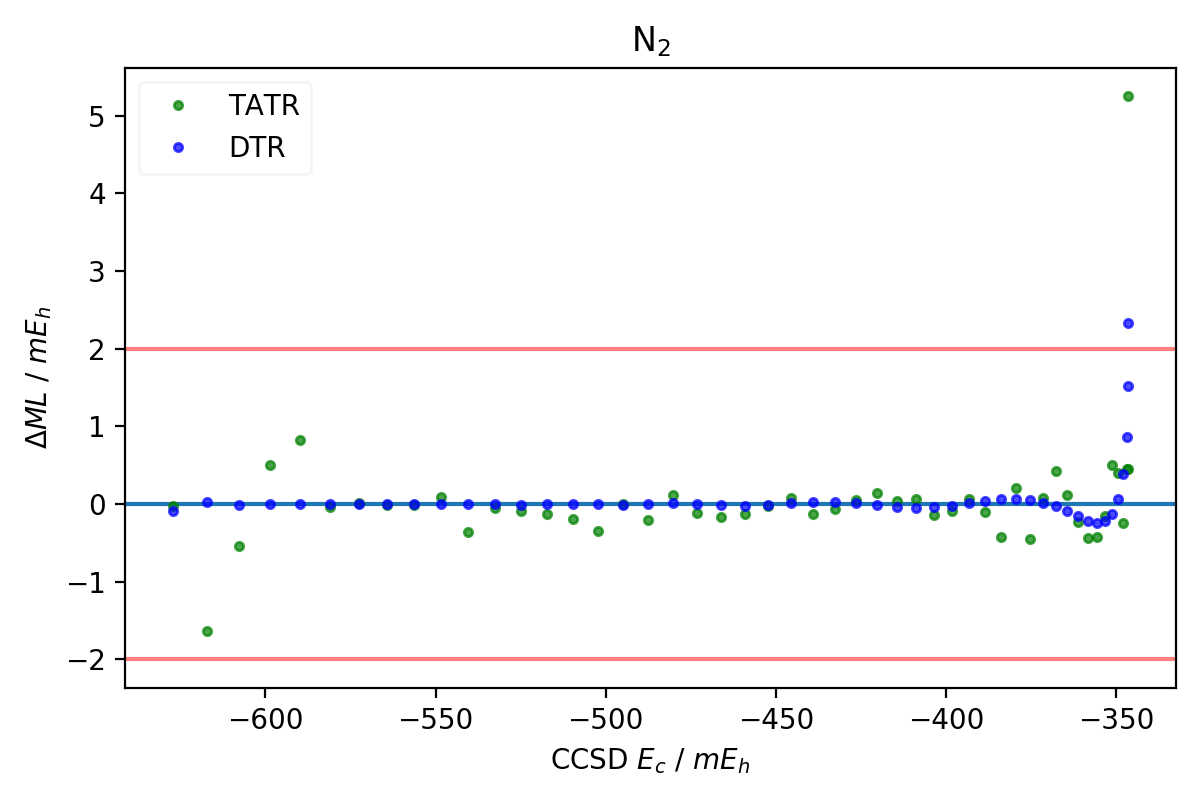
\includegraphics[scale=.55]{p2/figures/si/N2_e.png}
        \caption{}
        \label{fig:N2}
    \end{subfigure}
    \caption{DTR vs TATR errors in m$E_h$ for diatomic datasets: (a) H$_2$, (b) HF, (c) CO, (d) LiF, and (e) N$_2$. Red lines indicate 2 m$E_h$.}
    \label{fig:diatomics-E}
\end{figure}

\begin{figure}
    \begin{subfigure}{.5\textwidth}
        \centering
        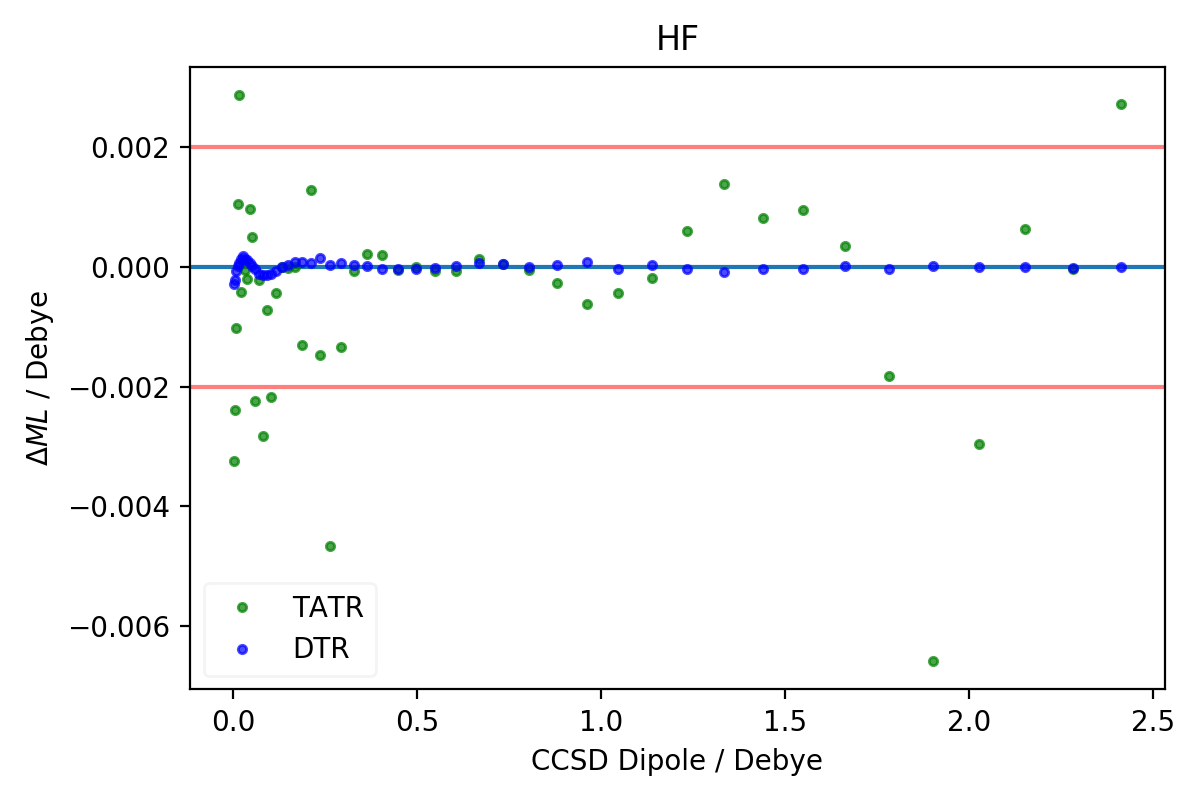
\includegraphics[scale=.55]{p2/figures/si/HF_d.png}
        \caption{}
        \label{fig:HF}
    \end{subfigure}%
    \begin{subfigure}{.5\textwidth}
        \centering
        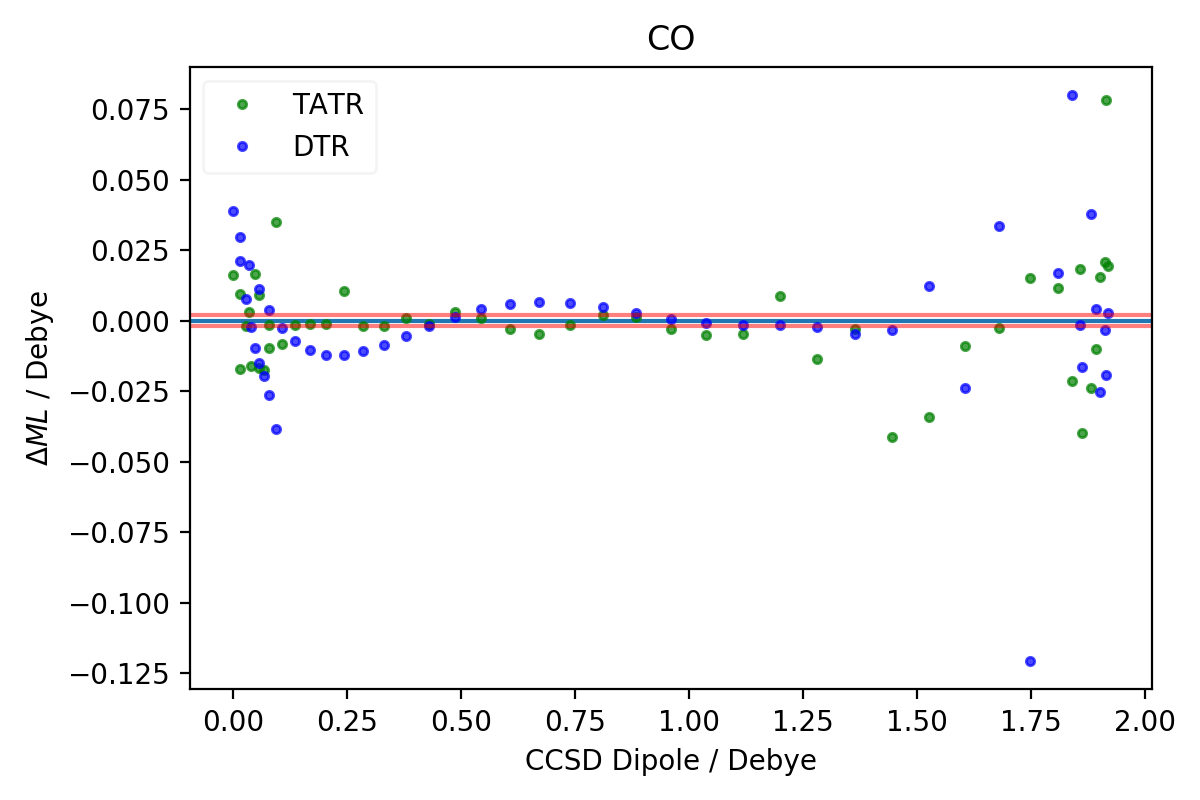
\includegraphics[scale=.55]{p2/figures/si/CO_d.png}
        \caption{}
        \label{fig:CO}
    \end{subfigure}
    \begin{subfigure}{.5\textwidth}
        \centering
        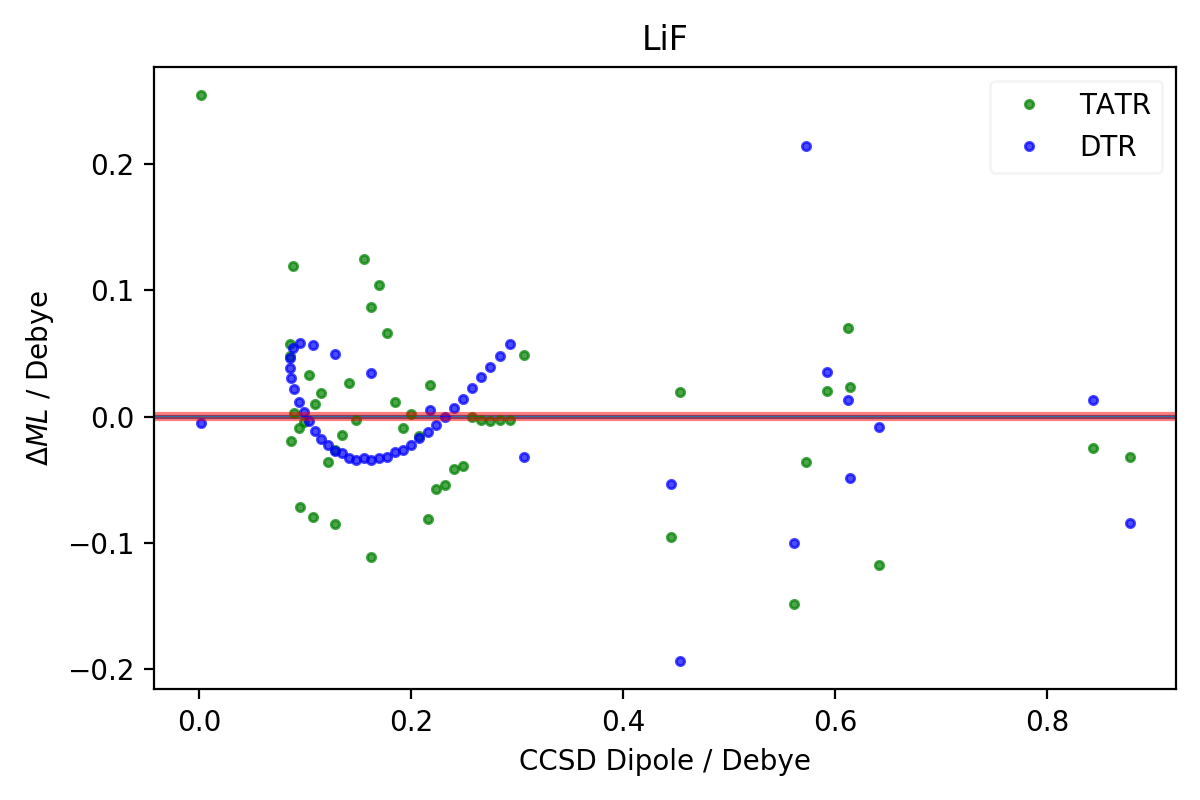
\includegraphics[scale=.55]{p2/figures/si/LiF_d.png}
        \caption{}
        \label{fig:LiF}
    \end{subfigure}
    \caption{DTR vs TATR errors in Debye for diatomic datasets: (a) HF, (b) CO, and (c) LiF. Red lines indicate 2 milliDebye.}
    \label{fig:diatomics-D}
\end{figure}

\begin{figure}
     \begin{subfigure}{.5\textwidth}
         \centering
         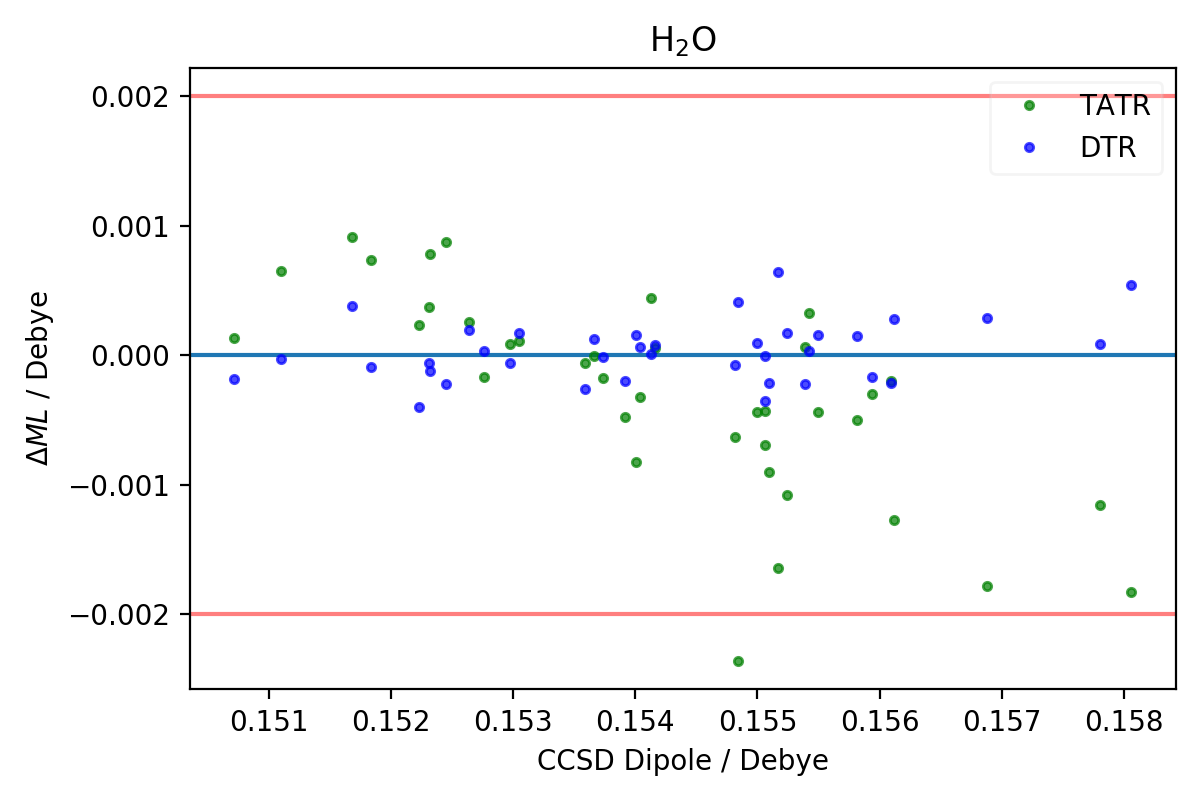
\includegraphics[scale=.55]{p2/figures/si/h2o_d.png}
         \caption{}
         \label{fig:H2O_D}
     \end{subfigure}%
     \begin{subfigure}{.5\textwidth}
         \centering
         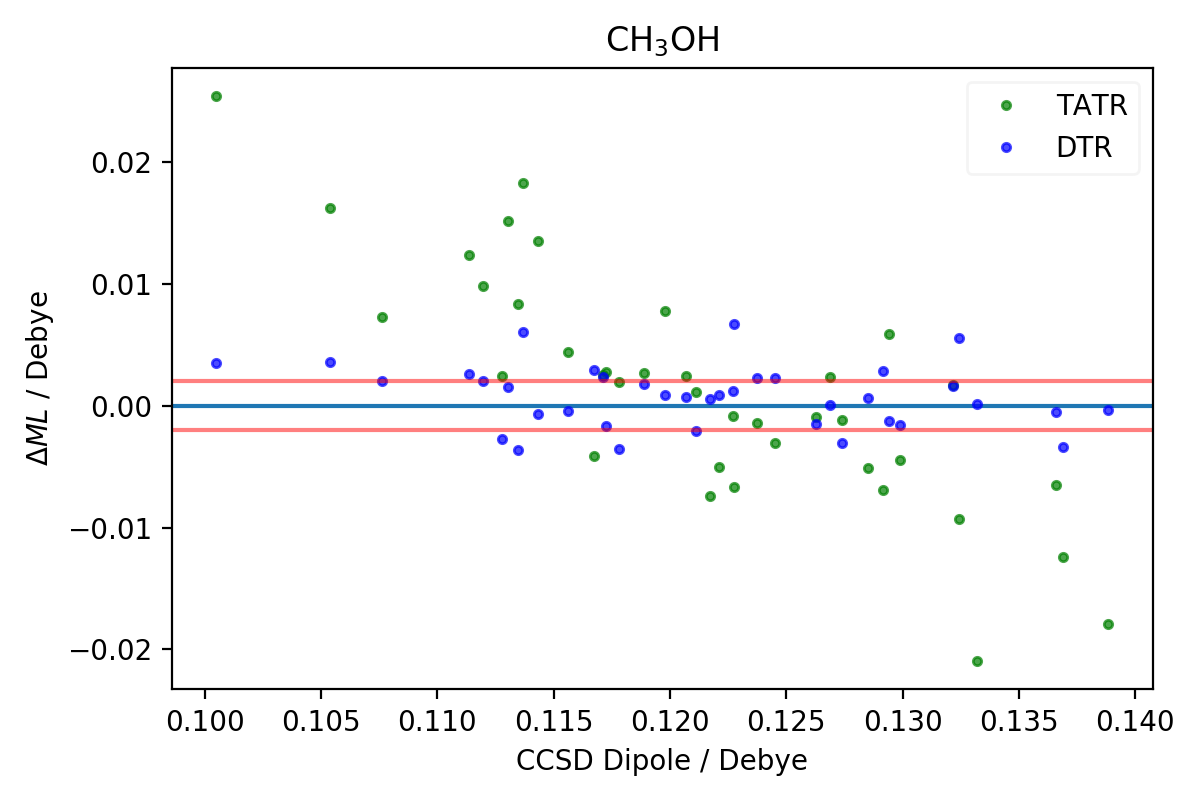
\includegraphics[scale=.55]{p2/figures/si/ch3oh_d.png}
         \caption{}
         \label{fig:CH3OH_D}
     \end{subfigure}
     \begin{subfigure}{.5\textwidth}
         \centering
         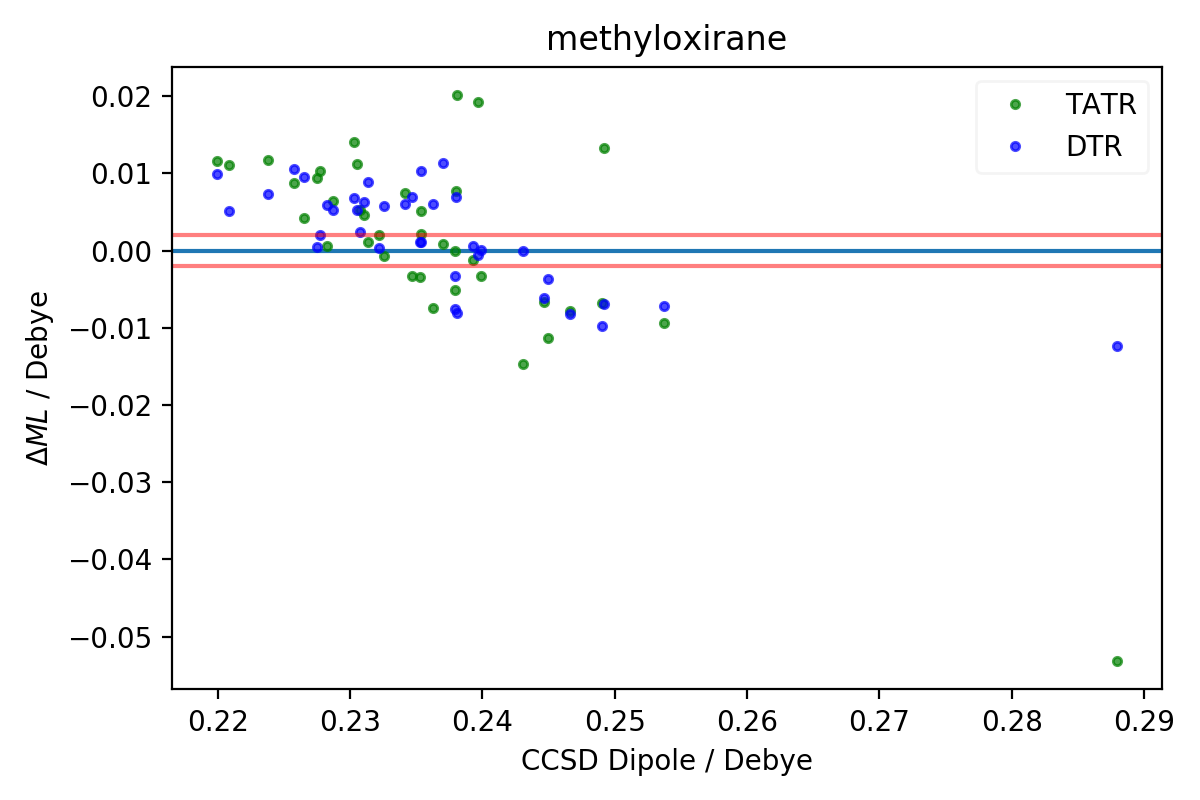
\includegraphics[scale=.55]{p2/figures/si/metox_d.png}
         \caption{}
         \label{fig:METOX_D}
     \end{subfigure}%
     \begin{subfigure}{.5\textwidth}
         \centering
         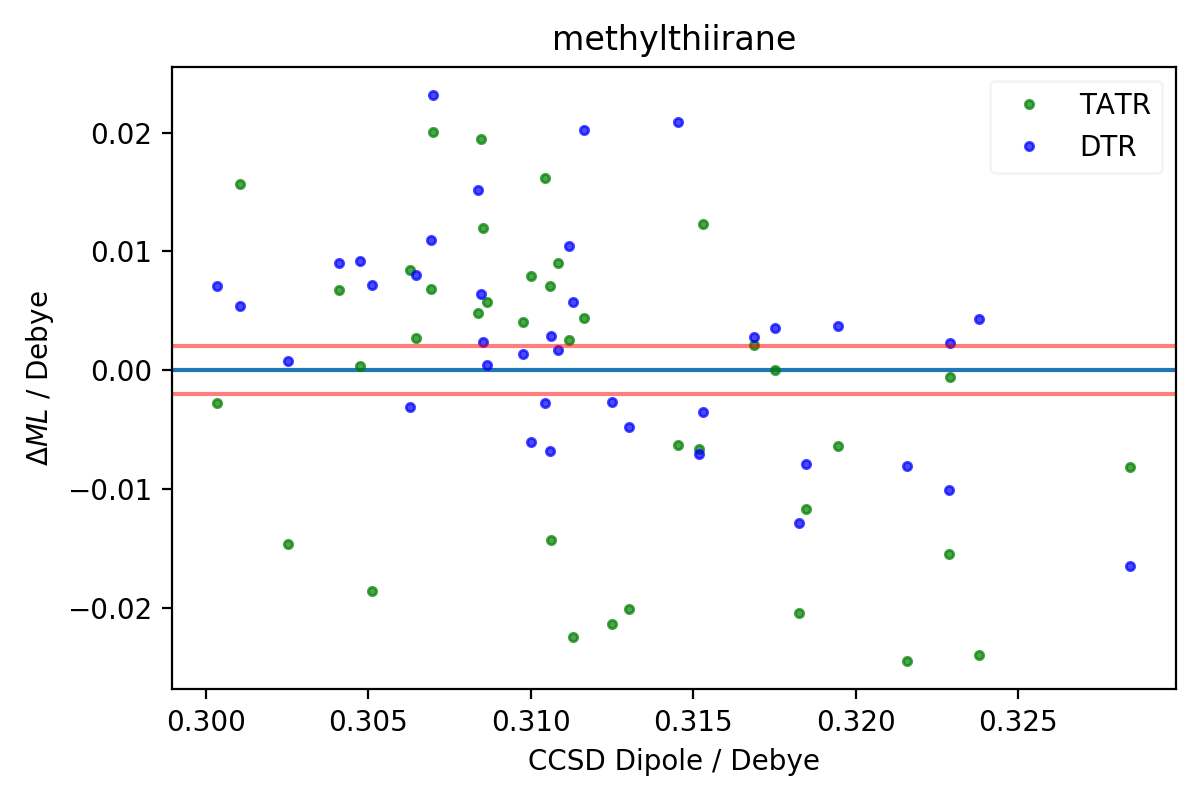
\includegraphics[scale=.55]{p2/figures/si/metthi_d.png}
         \caption{}
         \label{fig:METTHI_D}
     \end{subfigure}
     \caption{DTR vs TATR errors in Debye for small molecule datasets: (a) H$_2$O, (b) CH$_3$OH, (c) ($\textit{S}$)-methyloxirane, and (d) ($\textit{R}$)-methylthiirane. Red lines indicate 2 milliDebye.}
     \label{fig:small-D}
\end{figure}

\begin{figure}
    \centering
    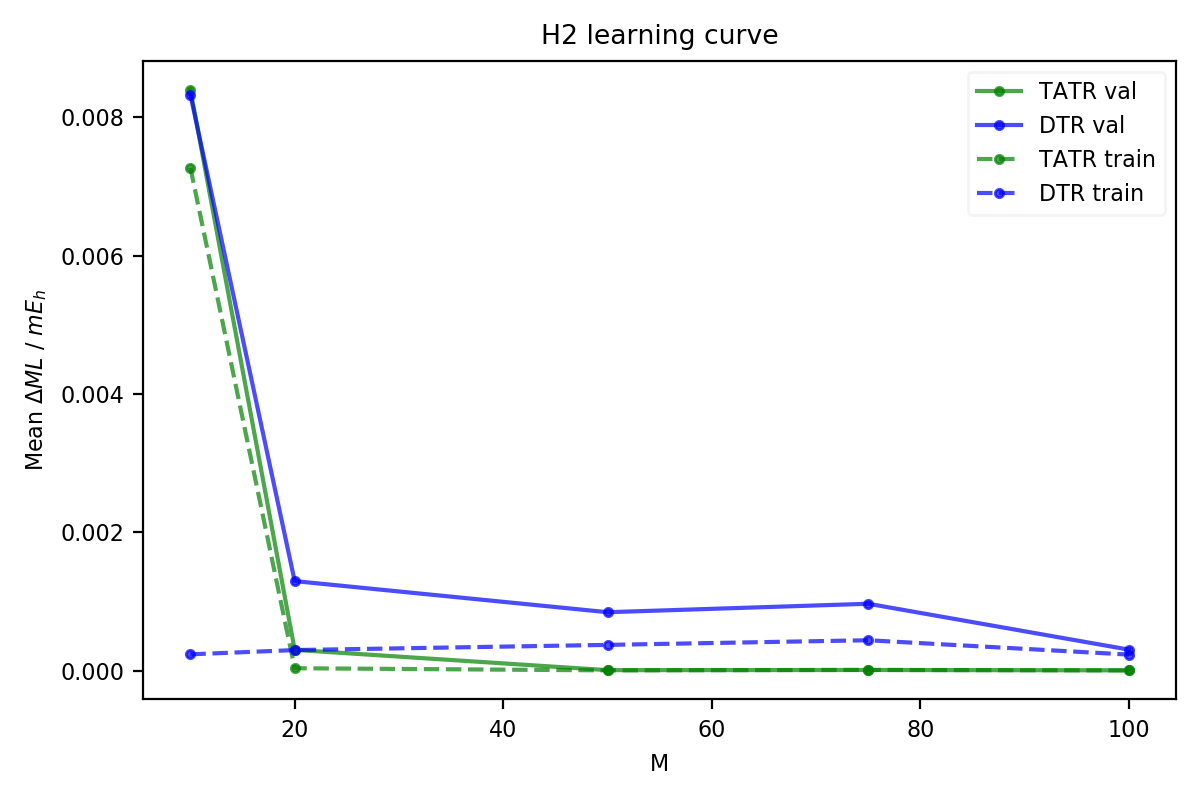
\includegraphics[scale=1.0]{p2/figures/si/H2_learn_e.png}
    \caption{DTR and TATR learning curves for H$_2$ correlation energy.}
\end{figure}

\begin{figure}
    \centering
    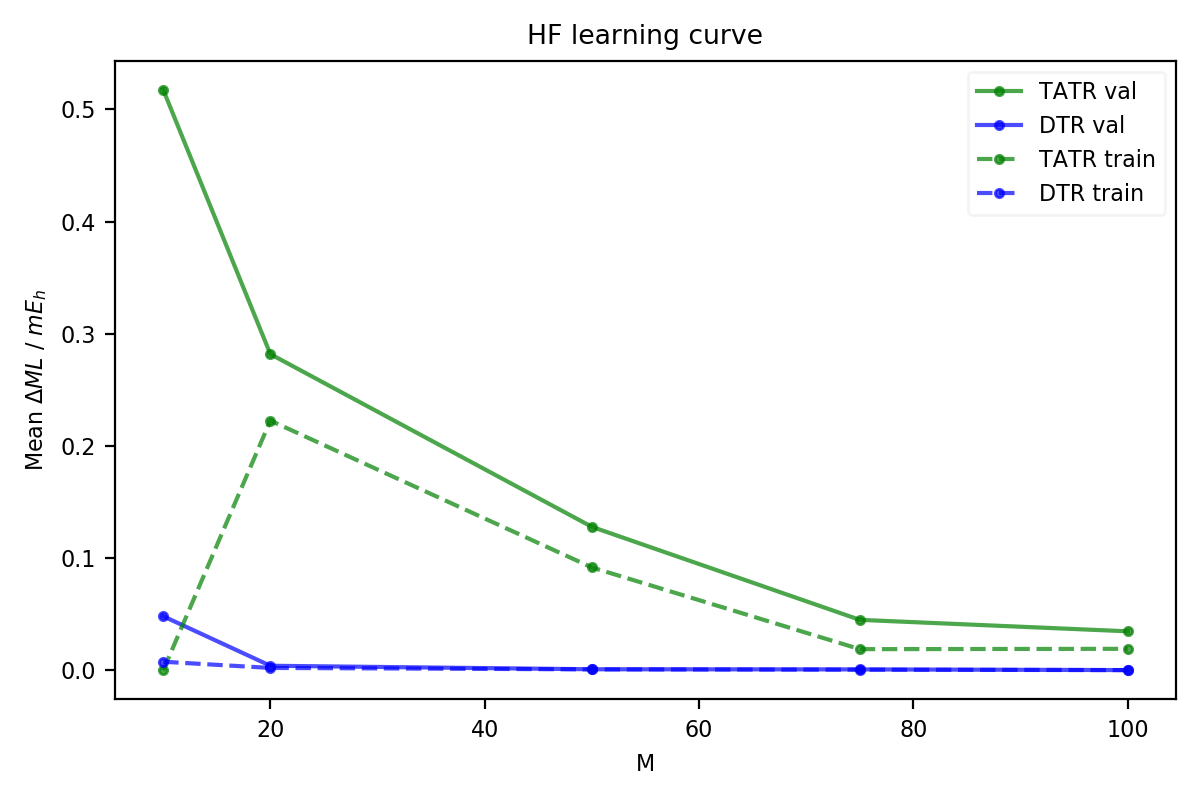
\includegraphics[scale=1.0]{p2/figures/si/HF_learn_e.png}
    \caption{DTR and TATR learning curves for HF correlation energy.}
\end{figure}

\begin{figure}
    \centering
    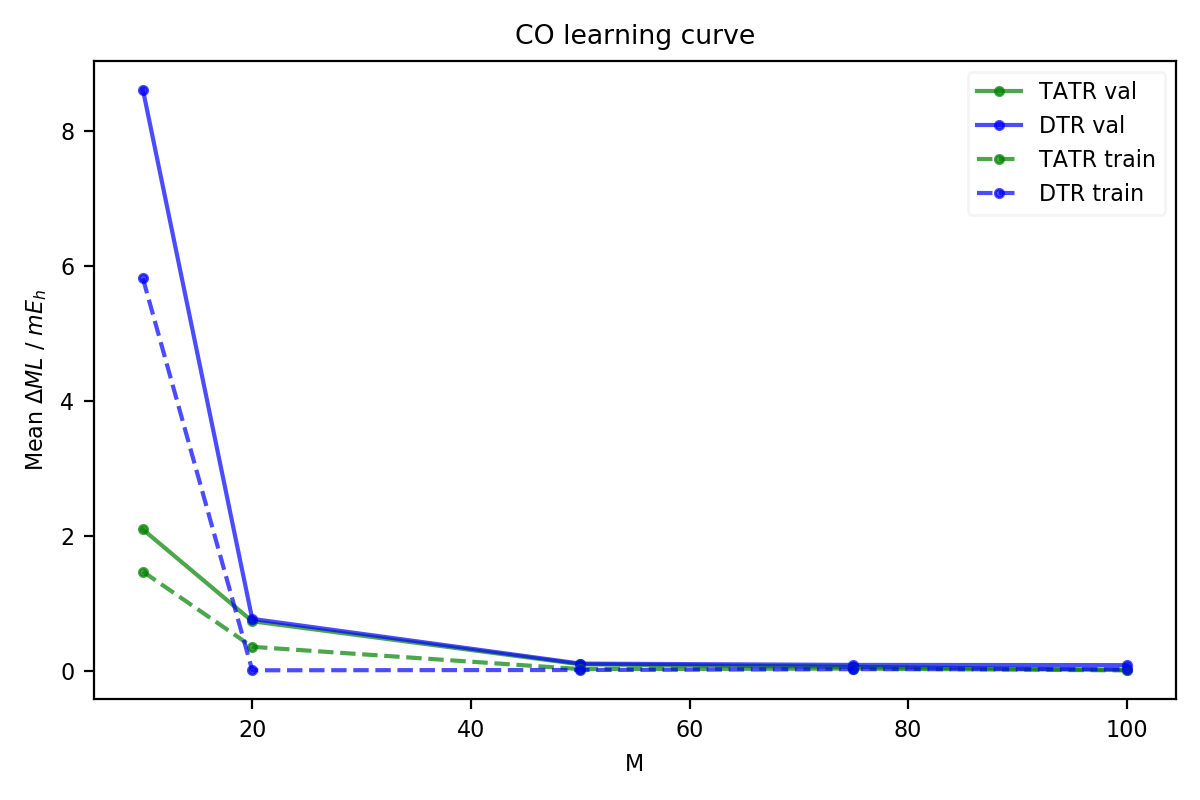
\includegraphics[scale=1.0]{p2/figures/si/CO_learn_e.png}
    \caption{DTR and TATR learning curves for CO correlation energy.}
\end{figure}

\begin{figure}
    \centering
    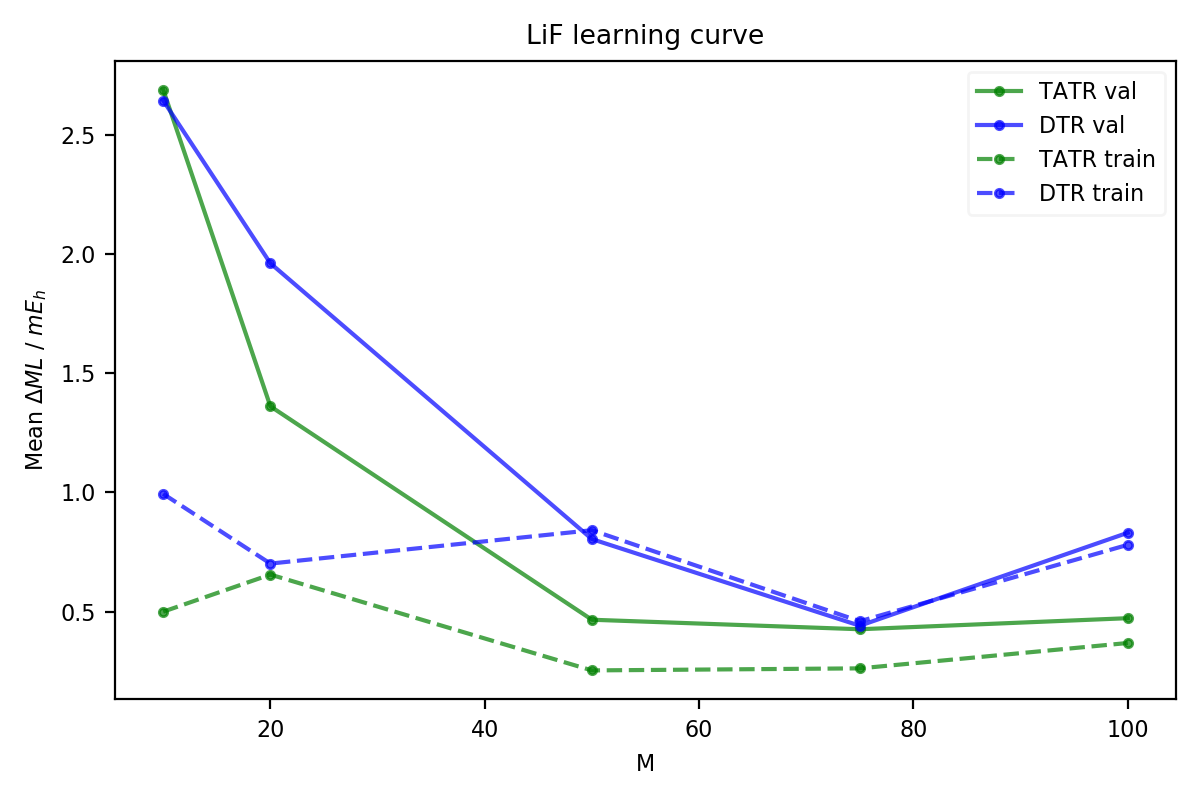
\includegraphics[scale=1.0]{p2/figures/si/LiF_learn_e.png}
    \caption{DTR and TATR learning curves for LiF correlation energy.}
\end{figure}

\begin{figure}
    \centering
    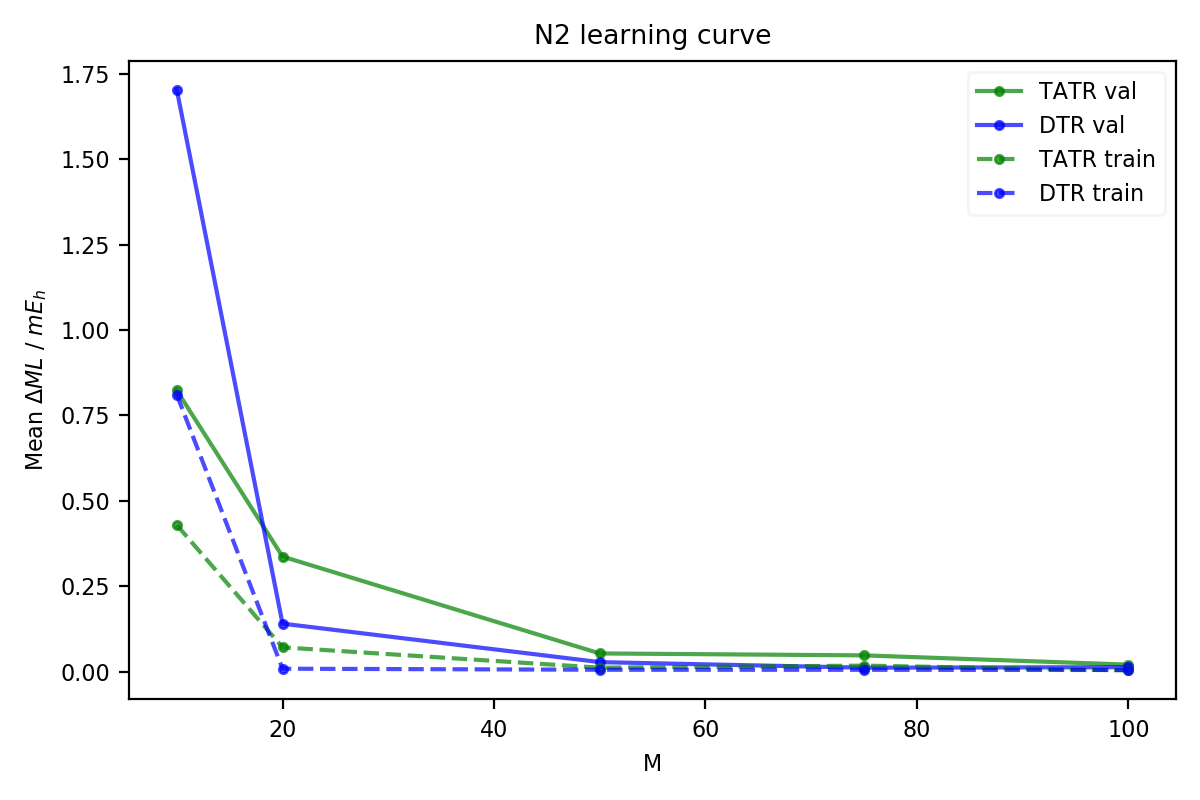
\includegraphics[scale=1.0]{p2/figures/si/N2_learn_e.png}
    \caption{DTR and TATR learning curves for N$_2$ correlation energy.}
\end{figure}

\begin{figure}
    \centering
    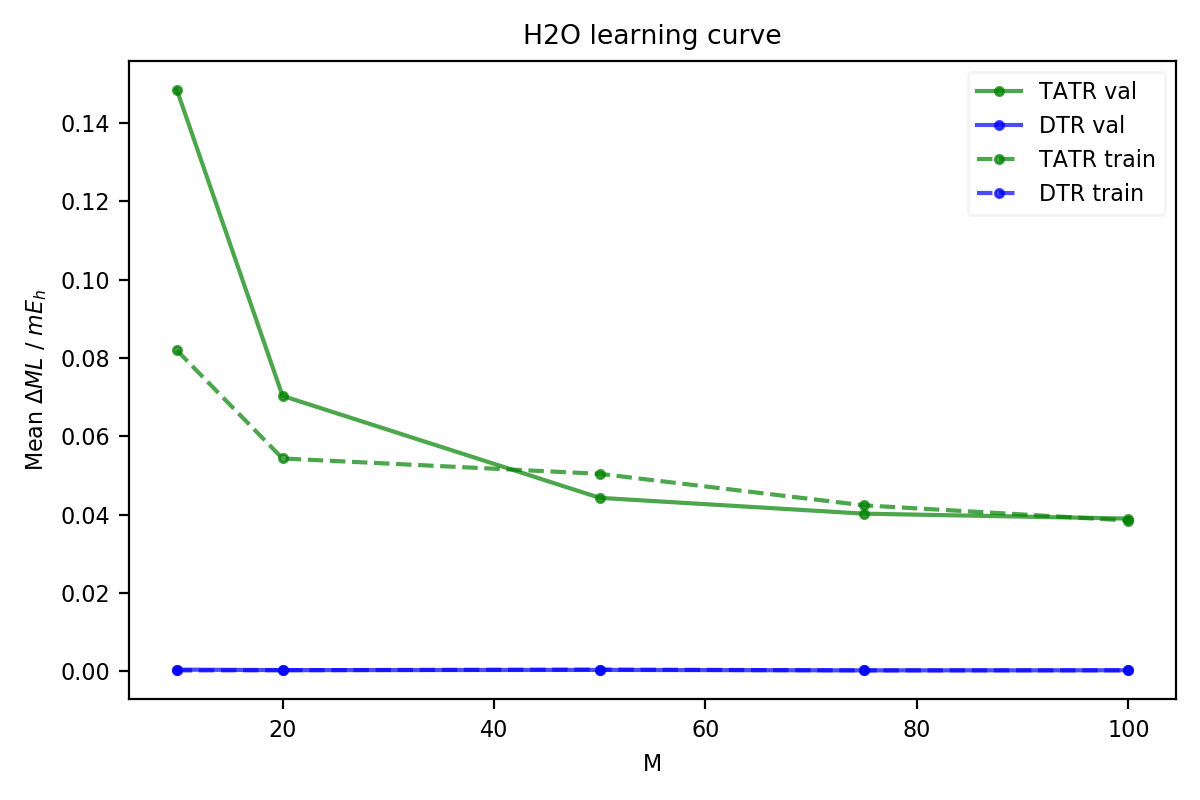
\includegraphics[scale=1.0]{p2/figures/si/H2O_learn_e.png}
    \caption{DTR and TATR learning curves for H$_2$O correlation energy.}
\end{figure}

\begin{figure}
    \centering
    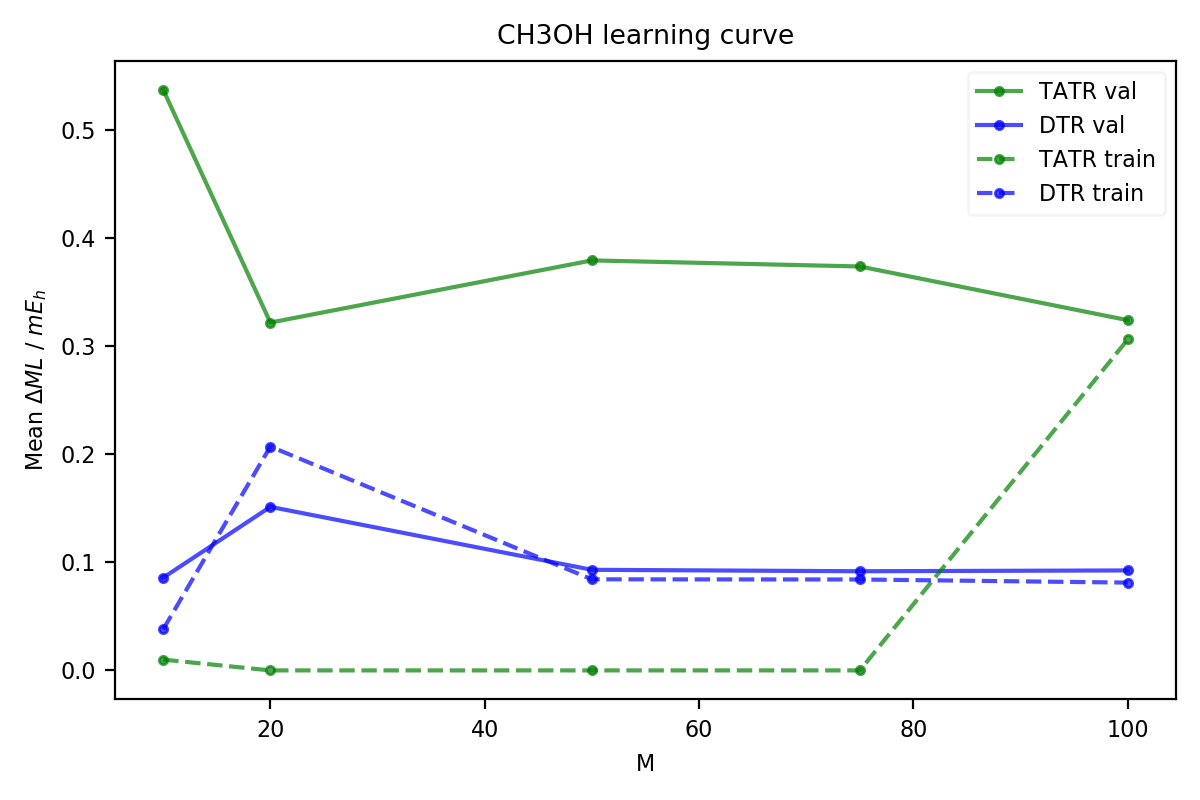
\includegraphics[scale=1.0]{p2/figures/si/CH3OH_learn_e.png}
    \caption{DTR and TATR learning curves for CH$_3$OH correlation energy.}
\end{figure}

\begin{figure}
    \centering
    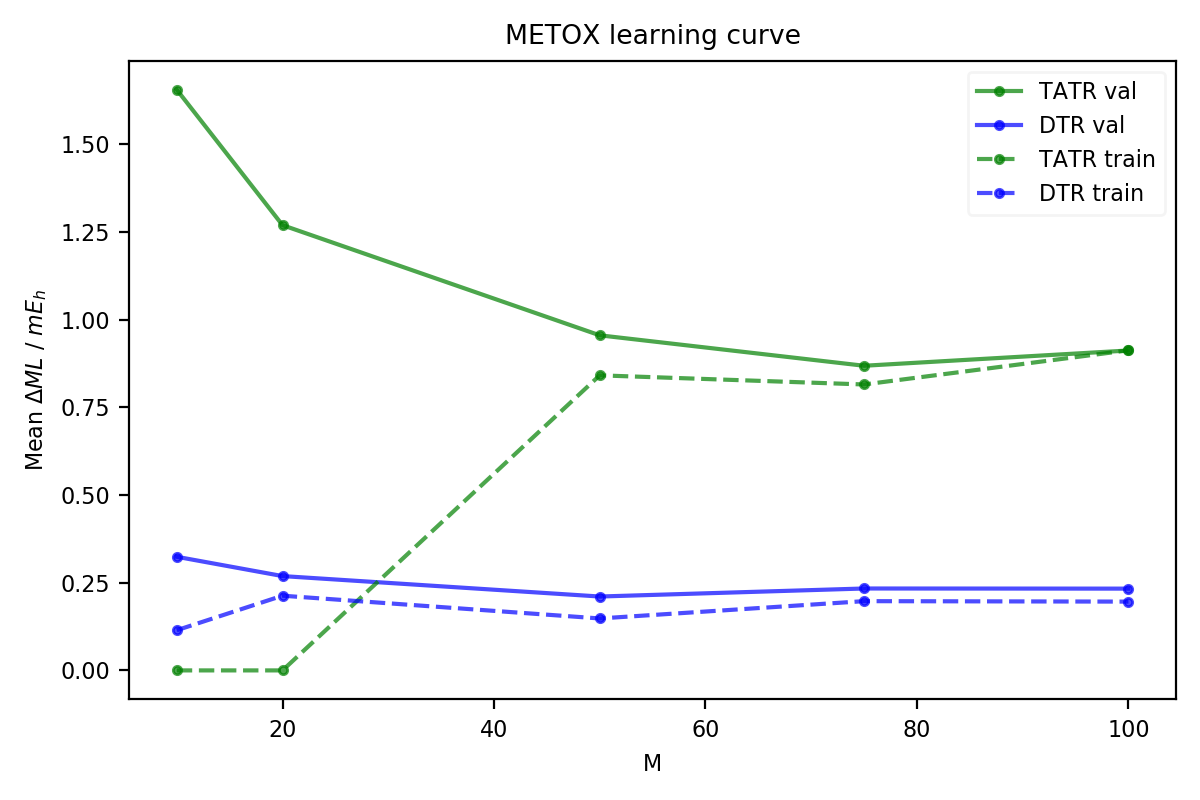
\includegraphics[scale=1.0]{p2/figures/si/METOX_learn_e.png}
    \caption{DTR and TATR learning curves for ($\textit{S}$)-methyloxirane correlation energy.}
\end{figure}

\begin{figure}
    \centering
    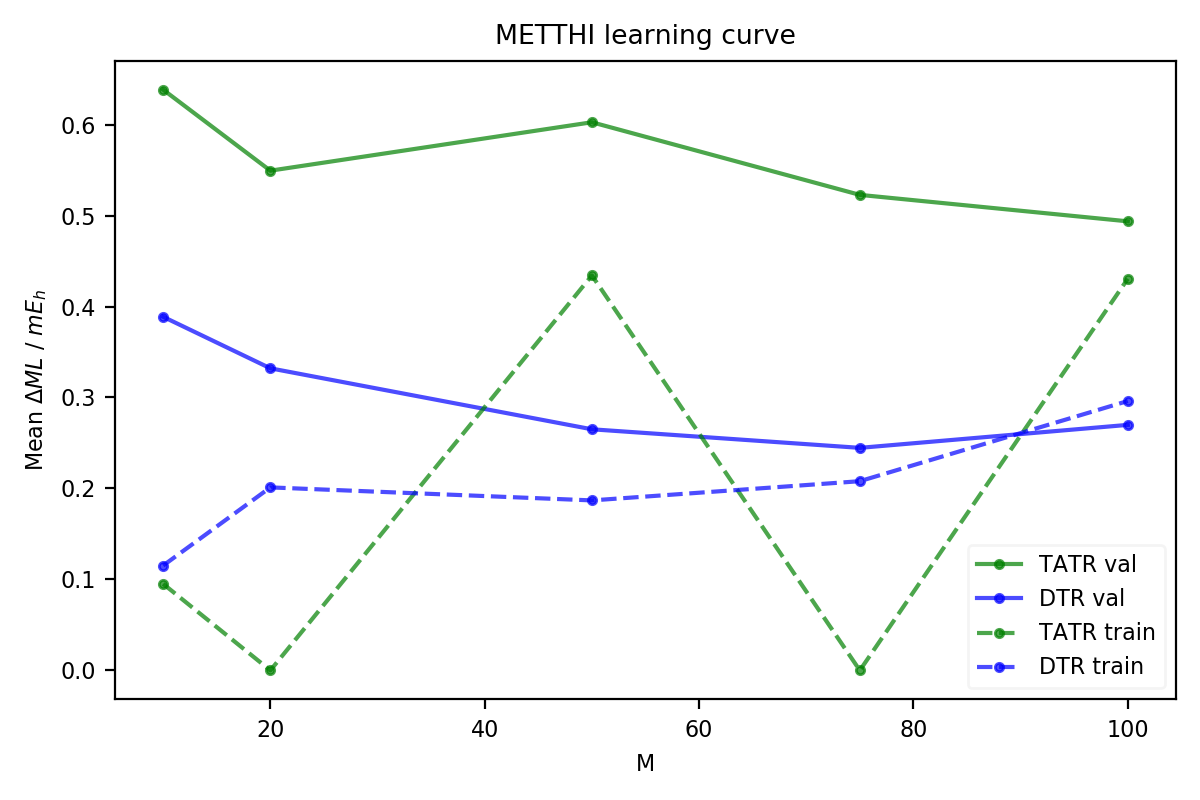
\includegraphics[scale=1.0]{p2/figures/si/METTHI_learn_e.png}
    \caption{DTR and TATR learning curves for ($\textit{R}$)-methylthiirane correlation energy.}
\end{figure}

\begin{figure}
    \centering
    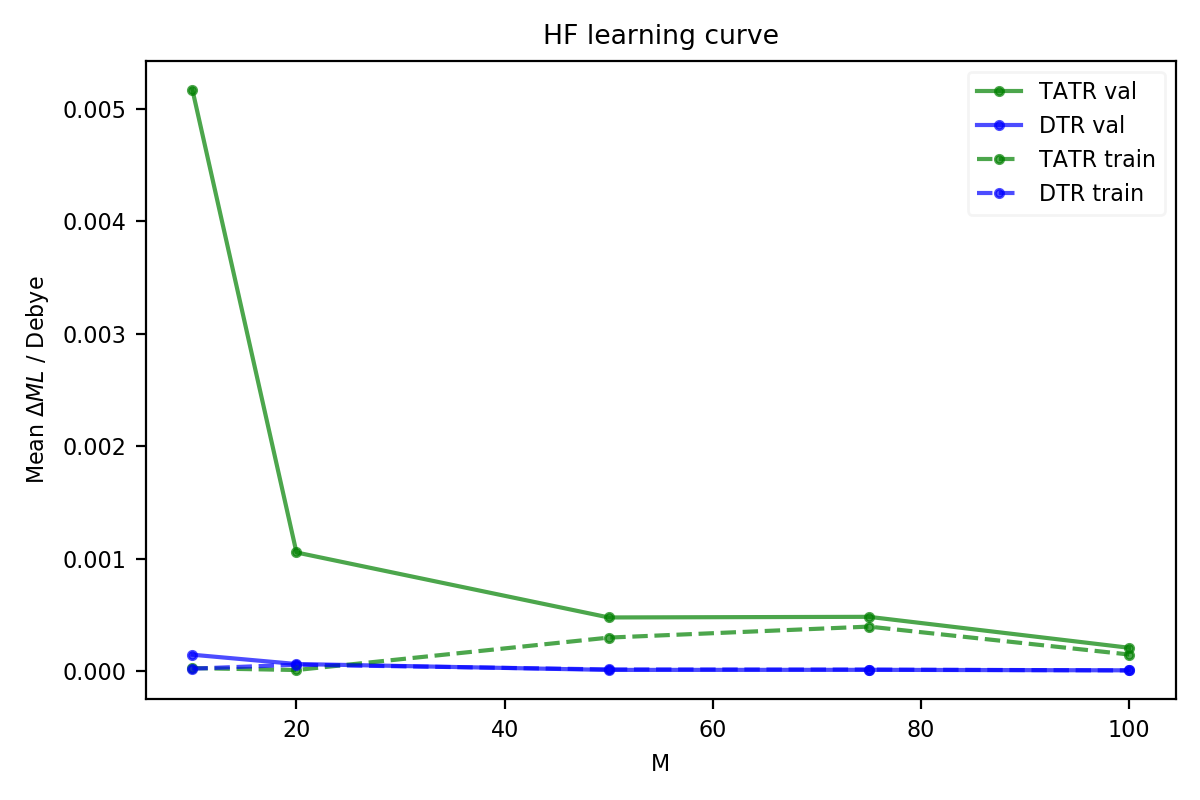
\includegraphics[scale=1.0]{p2/figures/si/HF_learn_d.png}
    \caption{DTR and TATR learning curves for HF correlated dipole.}
\end{figure}

\begin{figure}
    \centering
    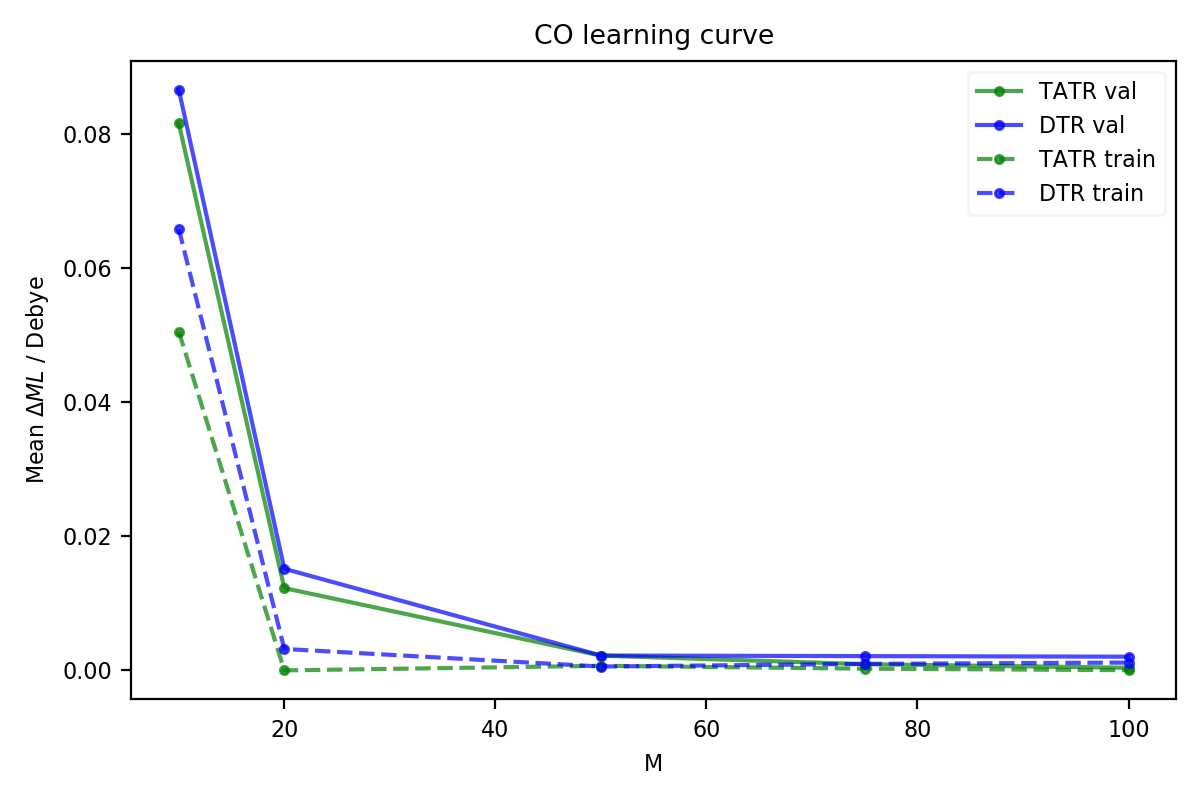
\includegraphics[scale=1.0]{p2/figures/si/CO_learn_d.png}
    \caption{DTR and TATR learning curves for CO correlated dipole.}
\end{figure}

\begin{figure}
    \centering
    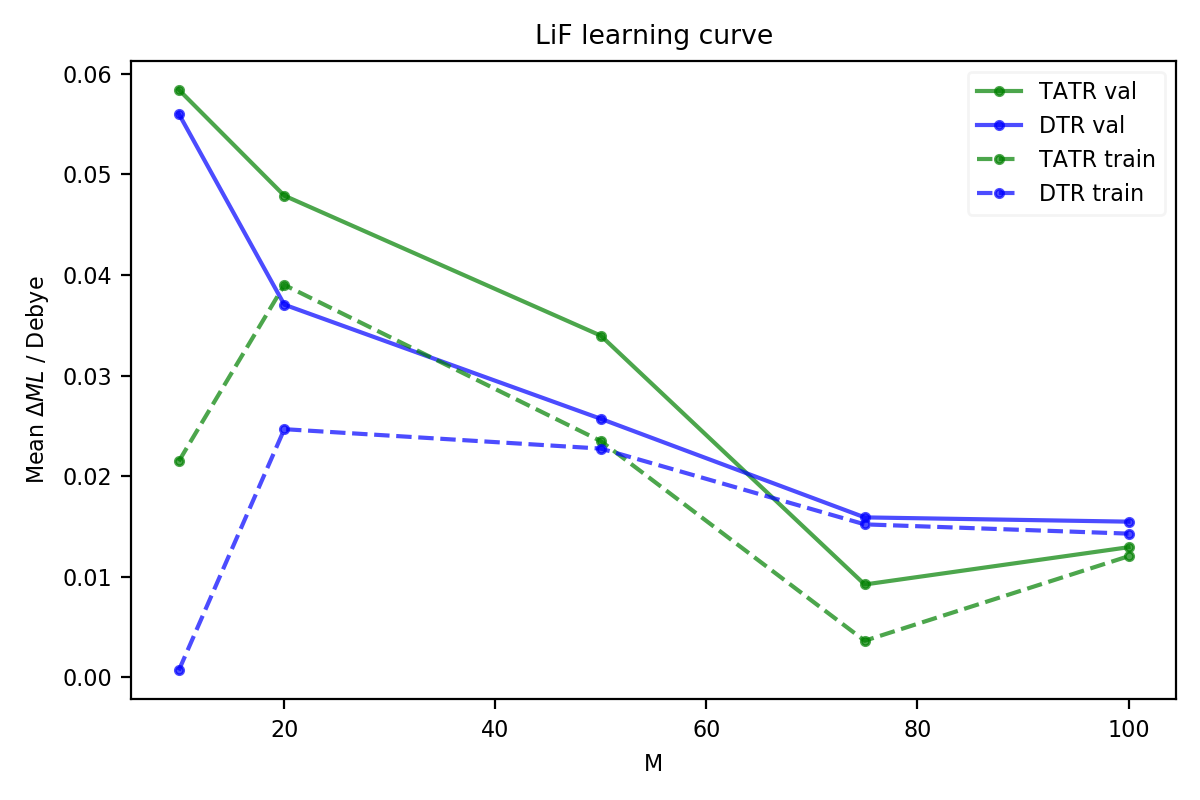
\includegraphics[scale=1.0]{p2/figures/si/LiF_learn_d.png}
    \caption{DTR and TATR learning curves for LiF correlated dipole.}
\end{figure}

\begin{figure}
    \centering
    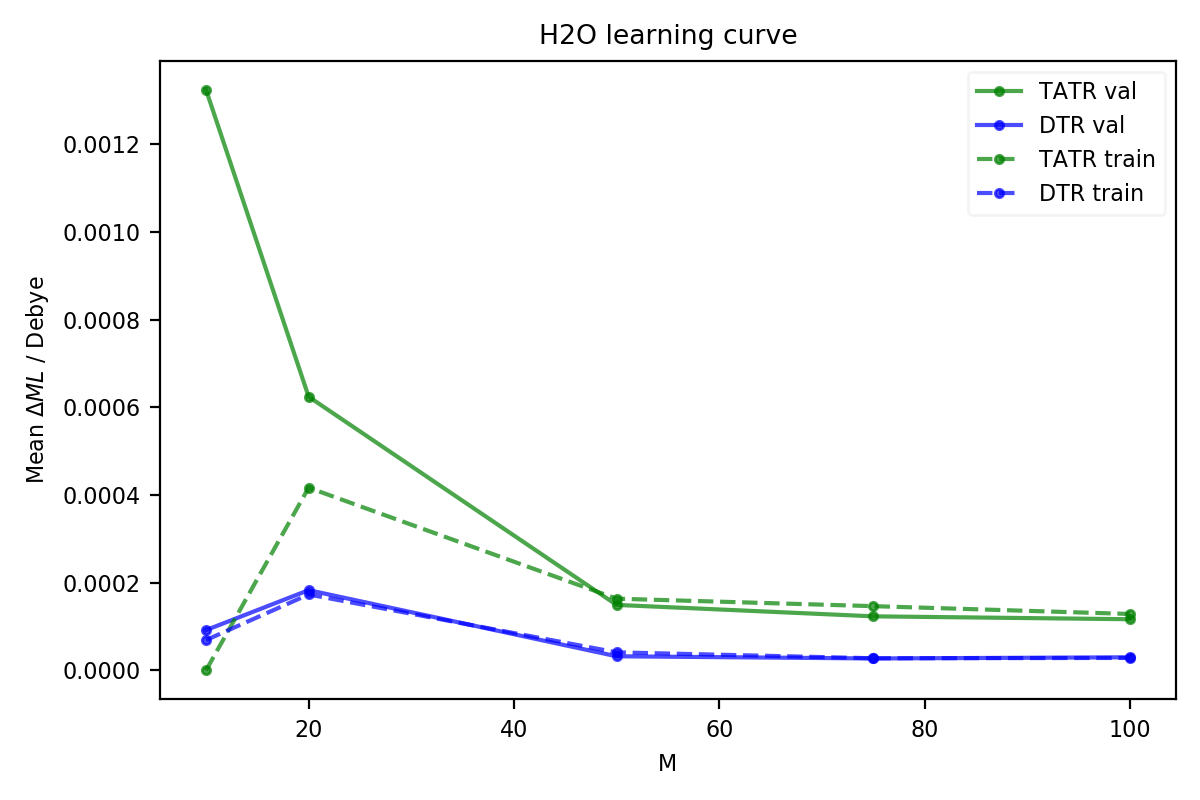
\includegraphics[scale=1.0]{p2/figures/si/H2O_learn_d.png}
    \caption{DTR and TATR learning curves for H$_2$O correlated dipole.}
\end{figure}

\begin{figure}
    \centering
    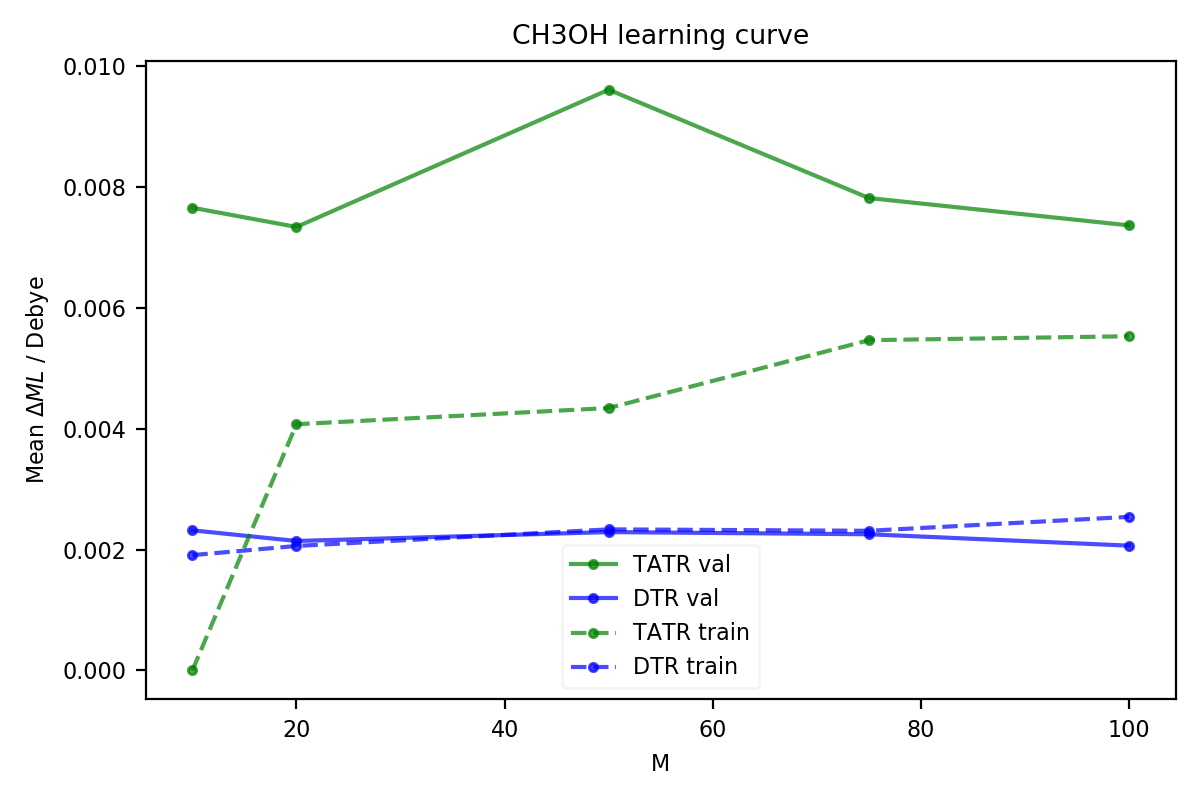
\includegraphics[scale=1.0]{p2/figures/si/CH3OH_learn_d.png}
    \caption{DTR and TATR learning curves for CH$_3$OH correlated dipole.}
\end{figure}

\begin{figure}
    \centering
    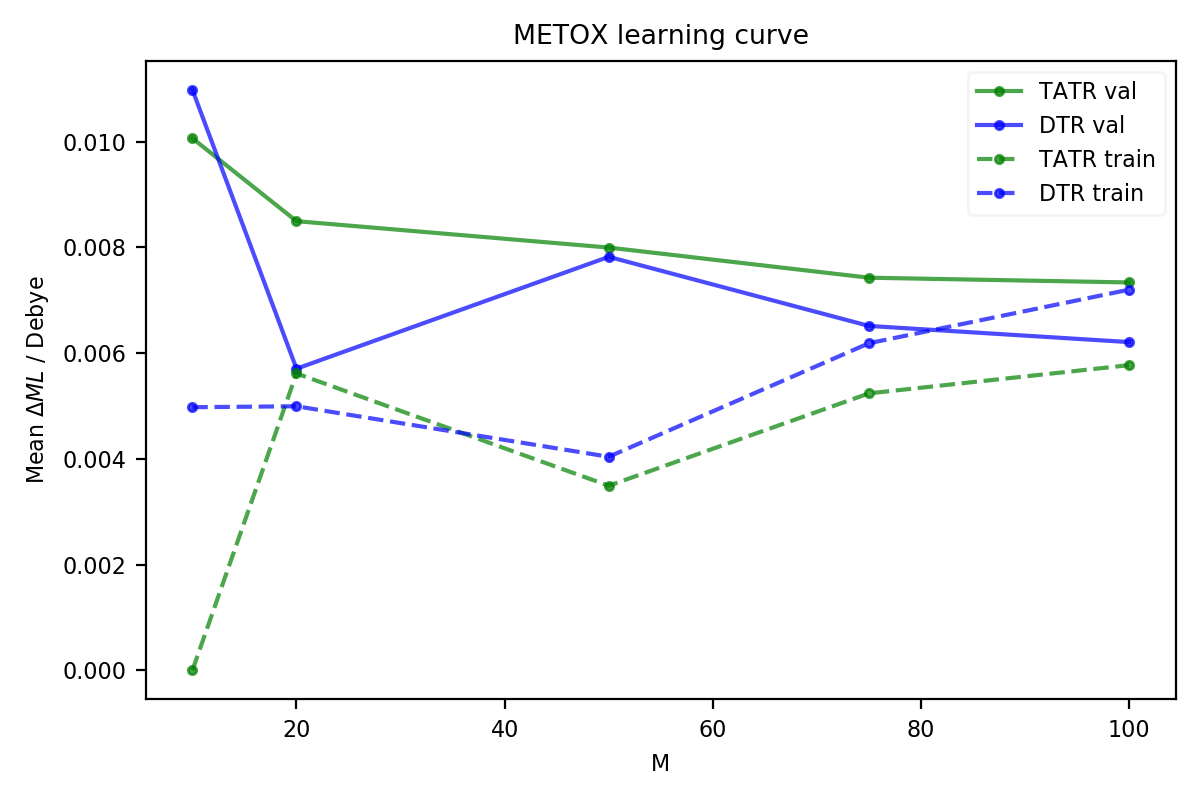
\includegraphics[scale=1.0]{p2/figures/si/METOX_learn_d.png}
    \caption{DTR and TATR learning curves for ($\textit{S}$)-methyloxirane correlated dipole.}
\end{figure}

\begin{figure}
    \centering
    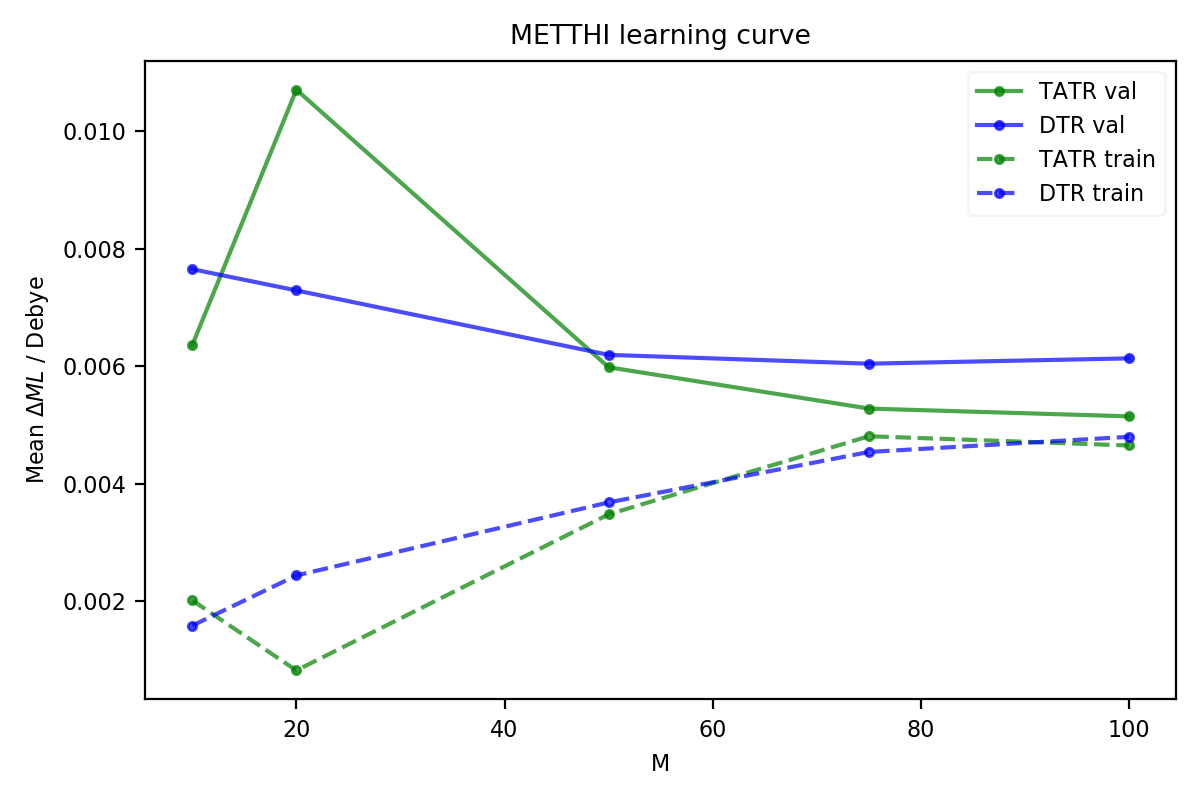
\includegraphics[scale=1.0]{p2/figures/si/METTHI_learn_d.png}
    \caption{DTR and TATR learning curves for ($\textit{R}$)-methylthiirane correlated dipole.}
\end{figure}

%%%%

\begin{figure}
    \centering
    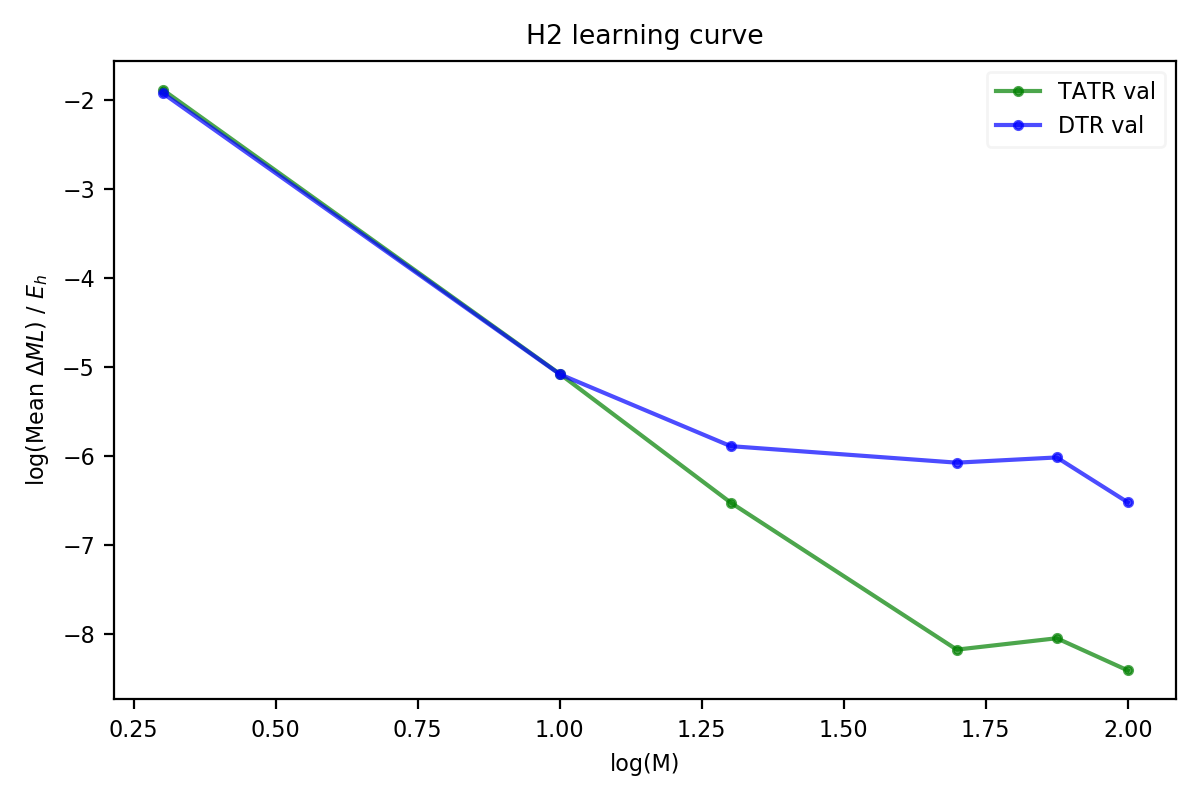
\includegraphics[scale=1.0]{p2/figures/si/H2_learn_log_e.png}
    \caption{DTR and TATR validation curves for H$_2$ correlation energy.}
\end{figure}

\begin{figure}
    \centering
    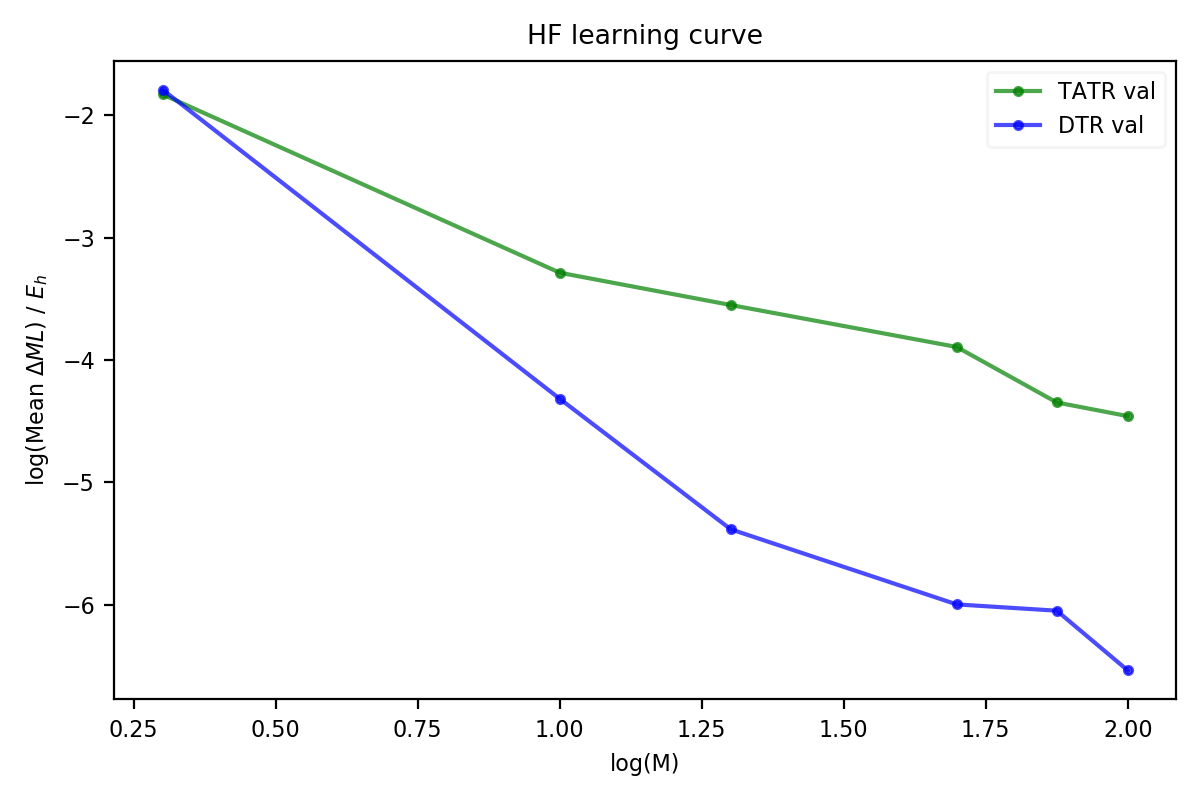
\includegraphics[scale=1.0]{p2/figures/si/HF_learn_log_e.png}
    \caption{DTR and TATR validation curves for HF correlation energy.}
\end{figure}

\begin{figure}
    \centering
    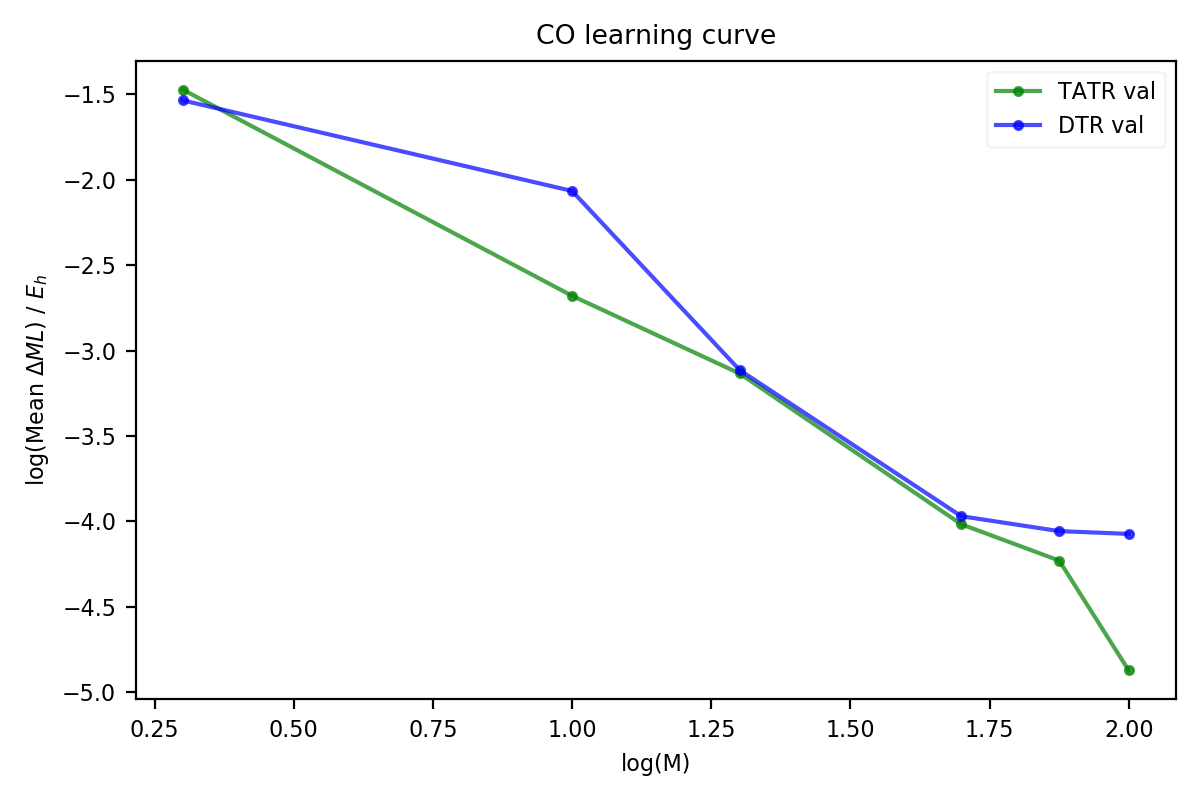
\includegraphics[scale=1.0]{p2/figures/si/CO_learn_log_e.png}
    \caption{DTR and TATR validation curves for CO correlation energy.}
\end{figure}

\begin{figure}
    \centering
    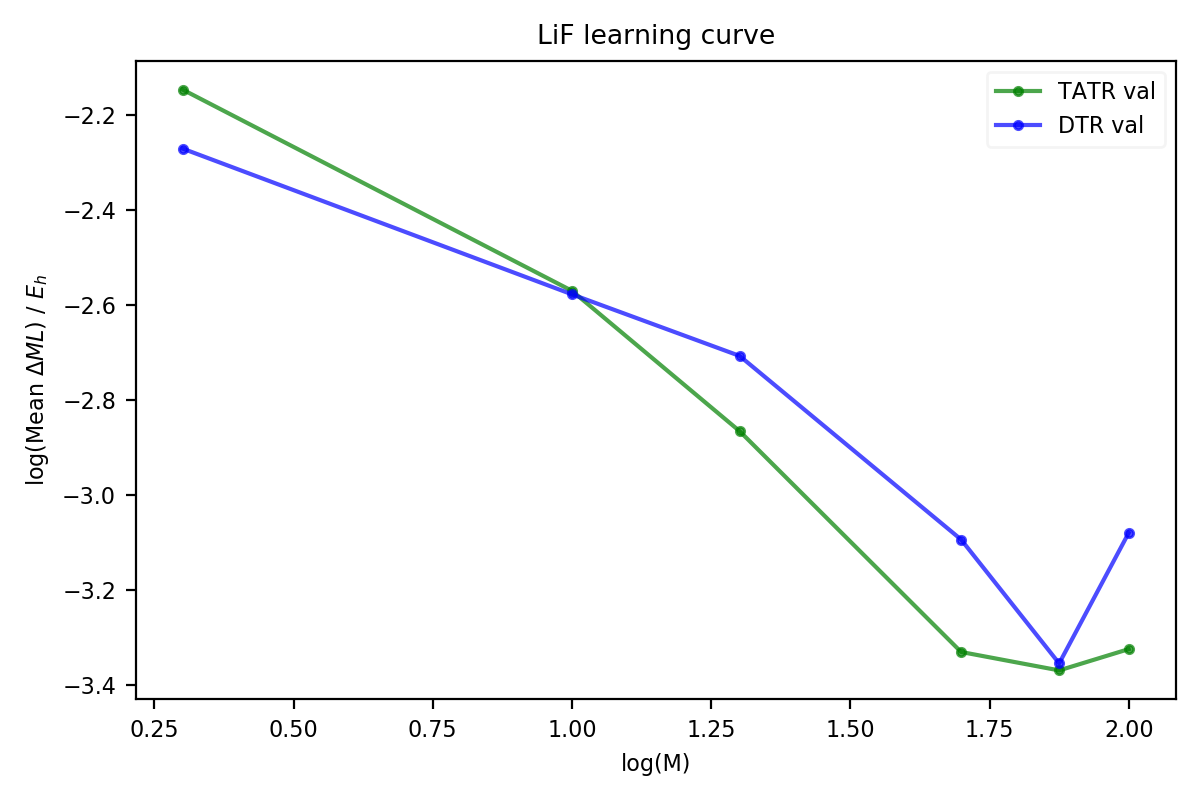
\includegraphics[scale=1.0]{p2/figures/si/LiF_learn_log_e.png}
    \caption{DTR and TATR validation curves for LiF correlation energy.}
\end{figure}

\begin{figure}
    \centering
    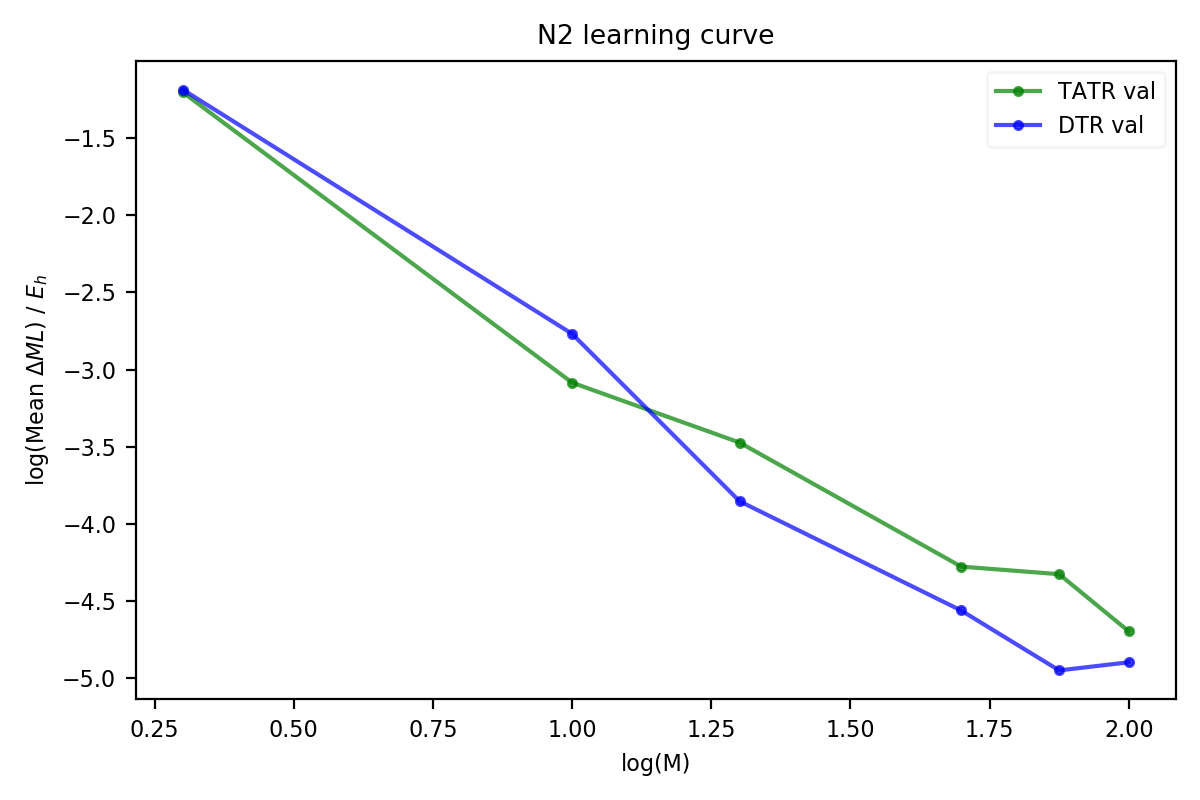
\includegraphics[scale=1.0]{p2/figures/si/N2_learn_log_e.png}
    \caption{DTR and TATR validation curves for N$_2$ correlation energy.}
\end{figure}

\begin{figure}
    \centering
    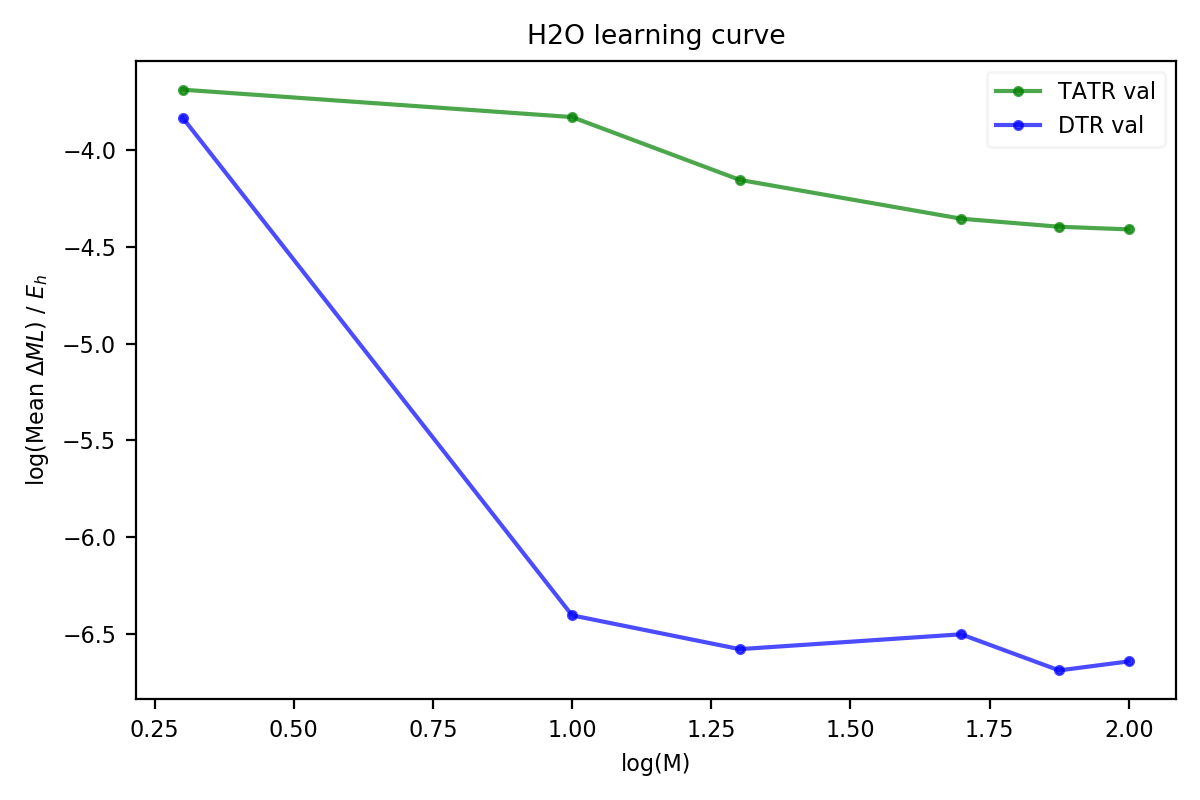
\includegraphics[scale=1.0]{p2/figures/si/H2O_learn_log_e.png}
    \caption{DTR and TATR validation curves for H$_2$O correlation energy.}
\end{figure}

\begin{figure}
    \centering
    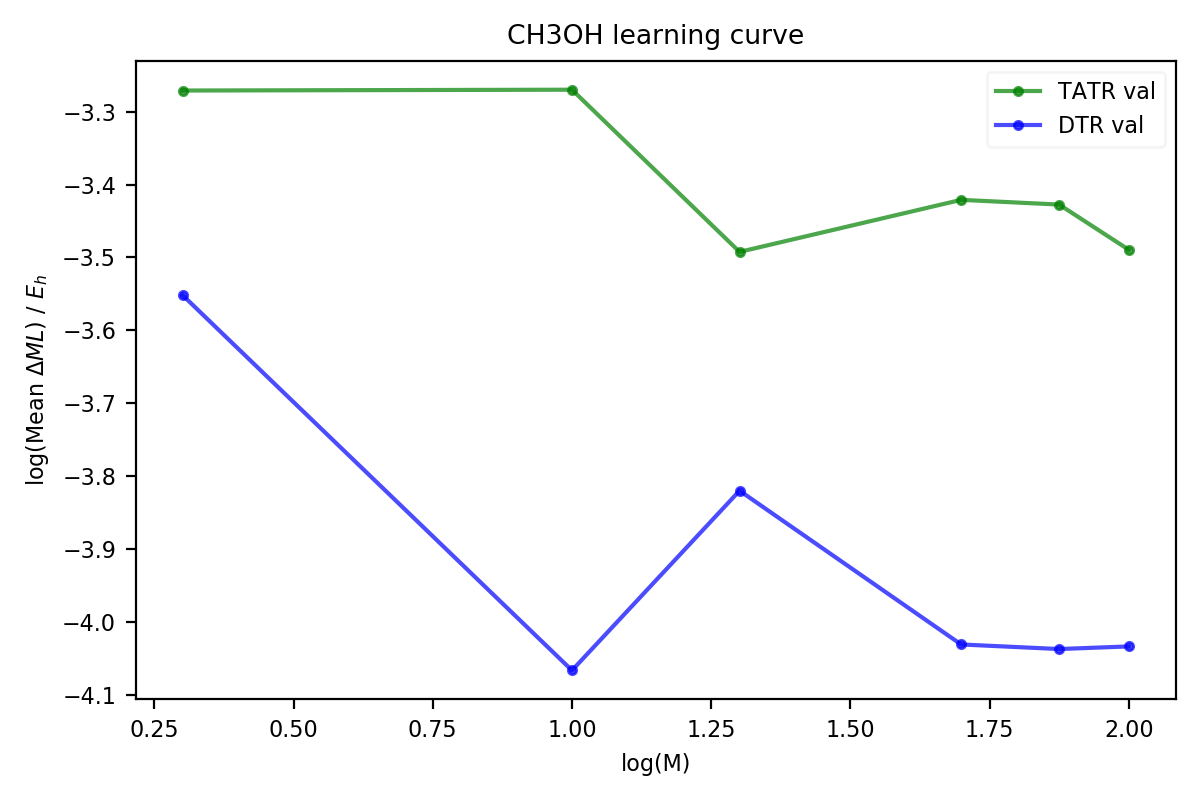
\includegraphics[scale=1.0]{p2/figures/si/CH3OH_learn_log_e.png}
    \caption{DTR and TATR validation curves for CH$_3$OH correlation energy.}
\end{figure}

\begin{figure}
    \centering
    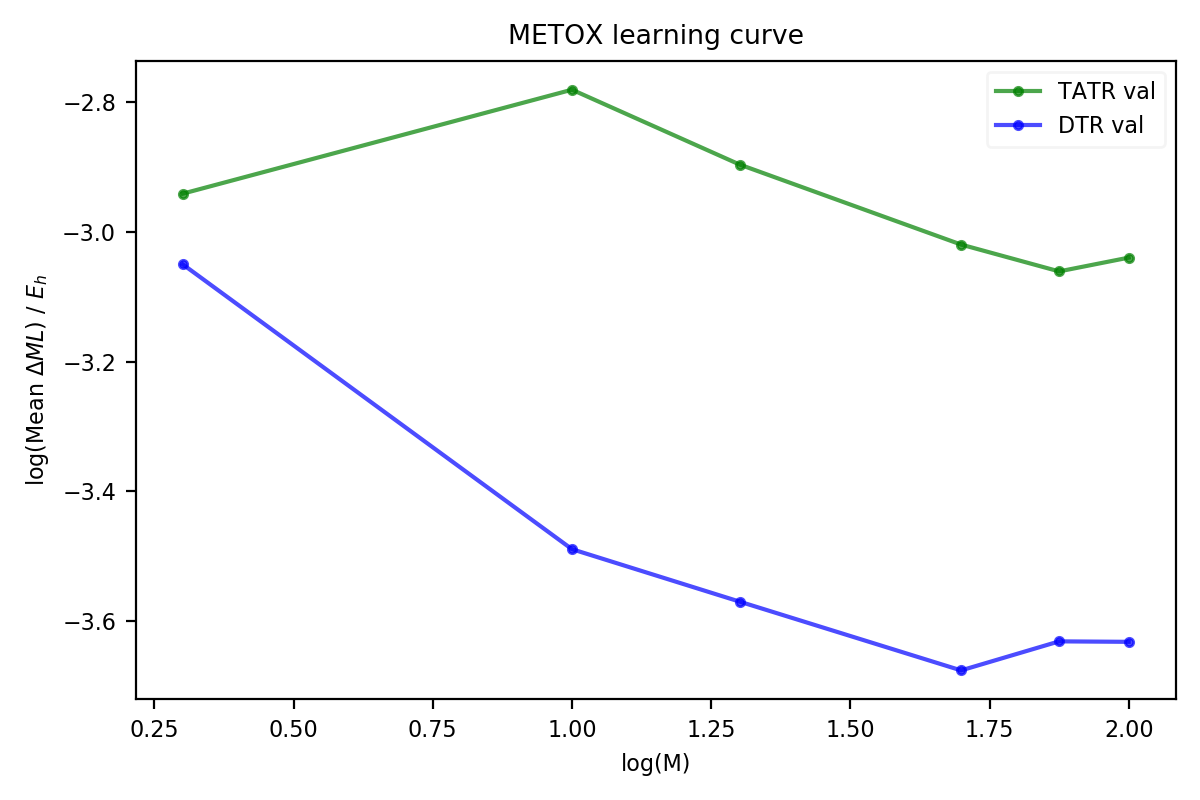
\includegraphics[scale=1.0]{p2/figures/si/METOX_learn_log_e.png}
    \caption{DTR and TATR validation curves for ($\textit{S}$)-methyloxirane correlation energy.}
\end{figure}

\begin{figure}
    \centering
    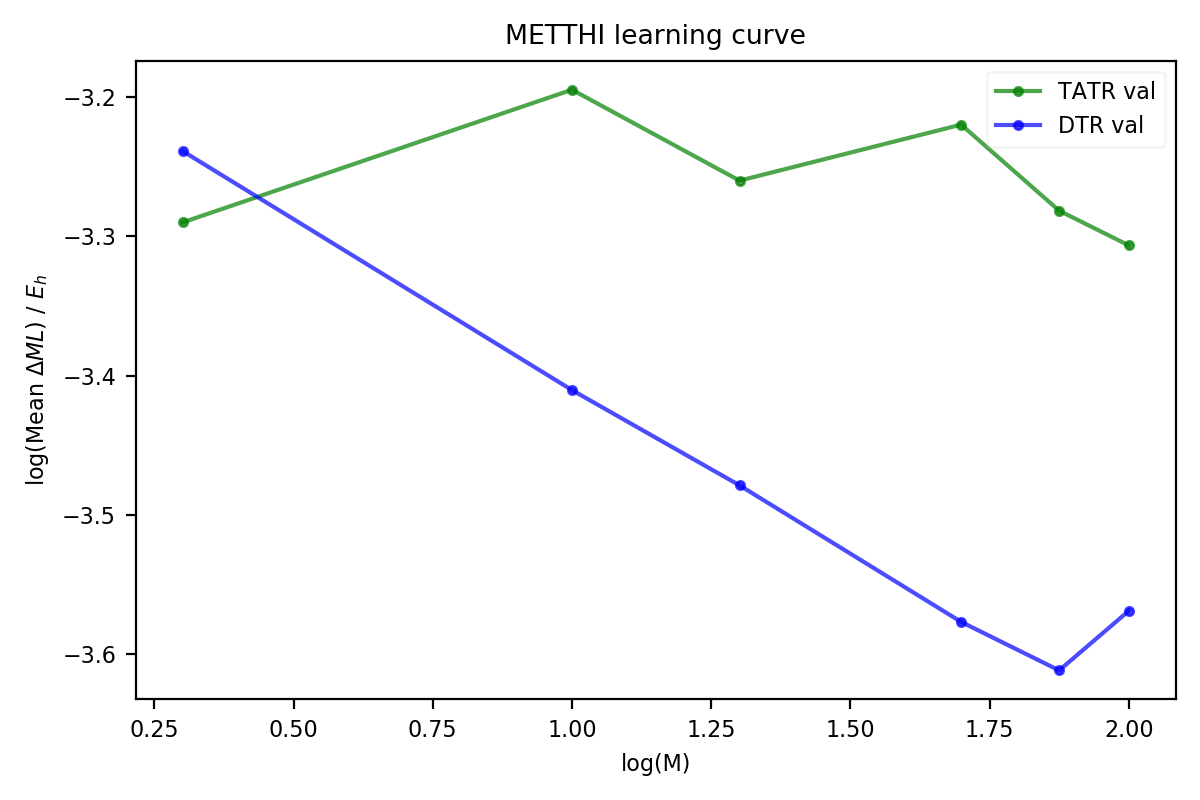
\includegraphics[scale=1.0]{p2/figures/si/METTHI_learn_log_e.png}
    \caption{DTR and TATR validation curves for ($\textit{R}$)-methylthiirane correlation energy.}
\end{figure}

\begin{figure}
    \centering
    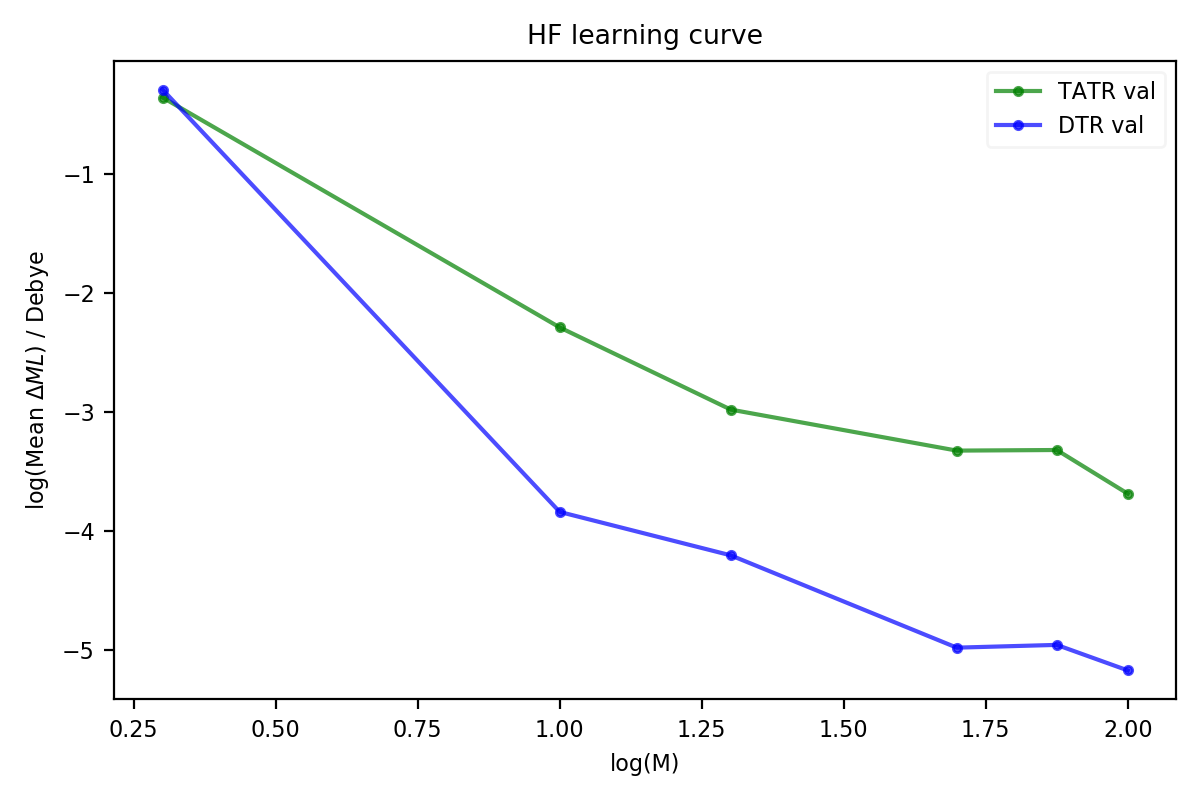
\includegraphics[scale=1.0]{p2/figures/si/HF_learn_log_d.png}
    \caption{DTR and TATR validation curves for HF correlated dipole.}
\end{figure}

\begin{figure}
    \centering
    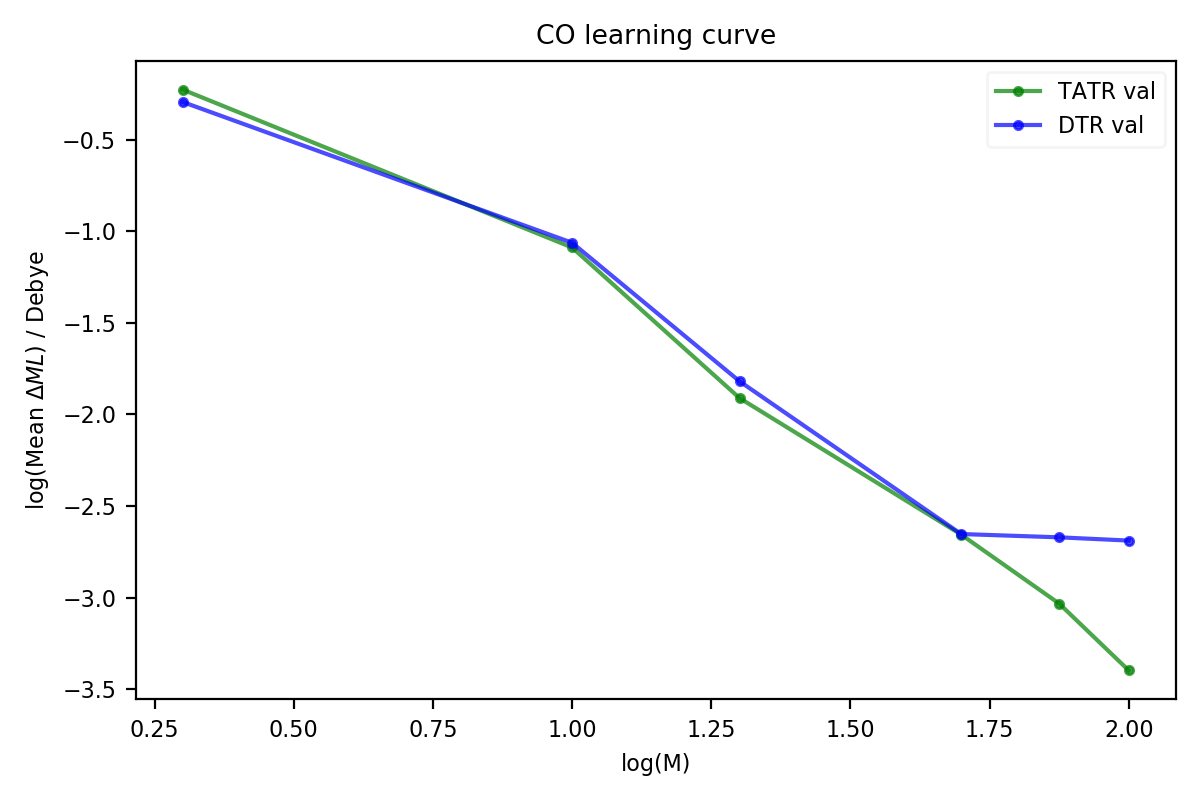
\includegraphics[scale=1.0]{p2/figures/si/CO_learn_log_d.png}
    \caption{DTR and TATR validation curves for CO correlated dipole.}
\end{figure}

\begin{figure}
    \centering
    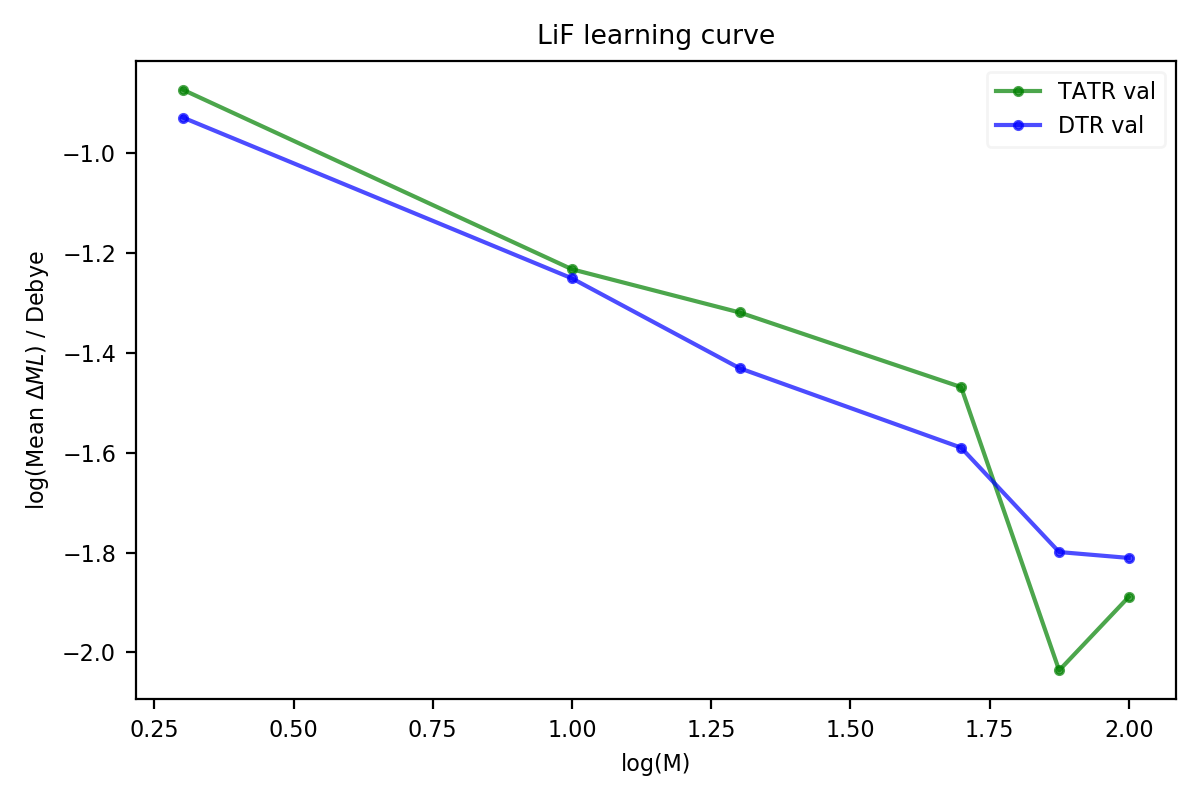
\includegraphics[scale=1.0]{p2/figures/si/LiF_learn_log_d.png}
    \caption{DTR and TATR validation curves for LiF correlated dipole.}
\end{figure}

\begin{figure}
    \centering
    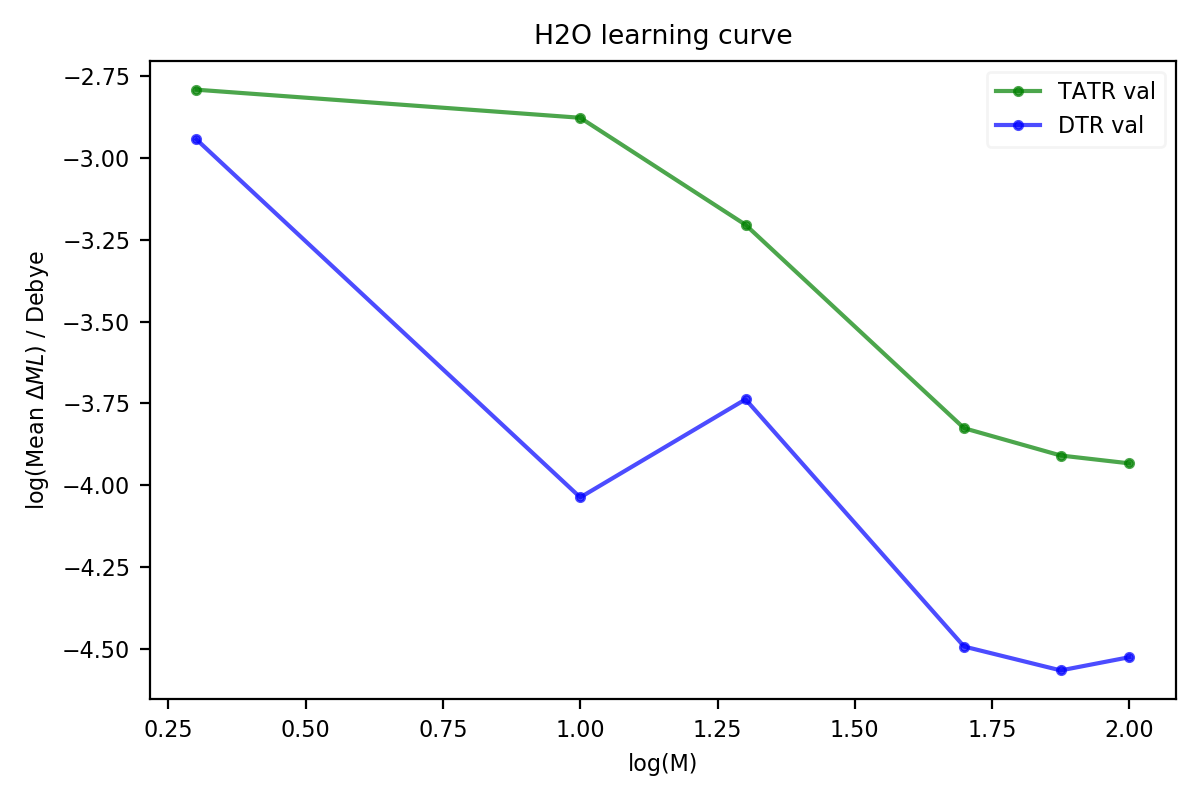
\includegraphics[scale=1.0]{p2/figures/si/H2O_learn_log_d.png}
    \caption{DTR and TATR validation curves for H$_2$O correlated dipole.}
\end{figure}

\begin{figure}
    \centering
    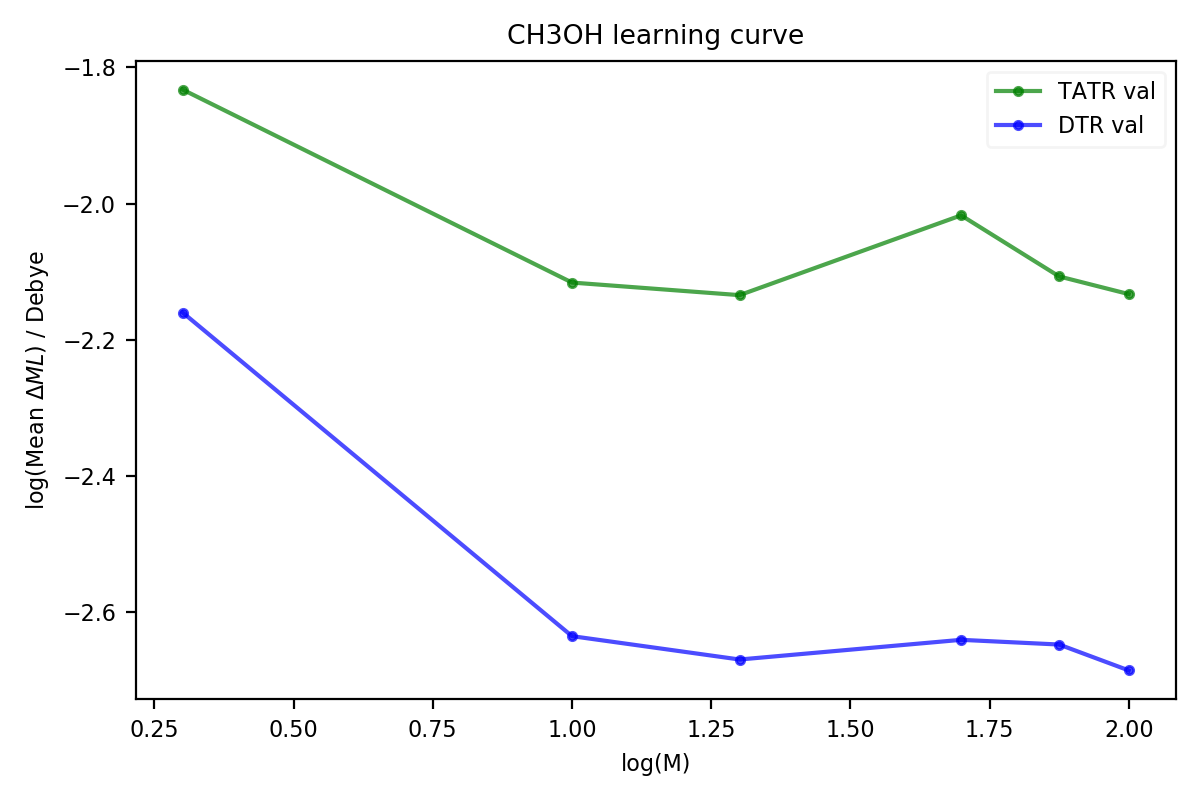
\includegraphics[scale=1.0]{p2/figures/si/CH3OH_learn_log_d.png}
    \caption{DTR and TATR validation curves for CH$_3$OH correlated dipole.}
\end{figure}

\begin{figure}
    \centering
    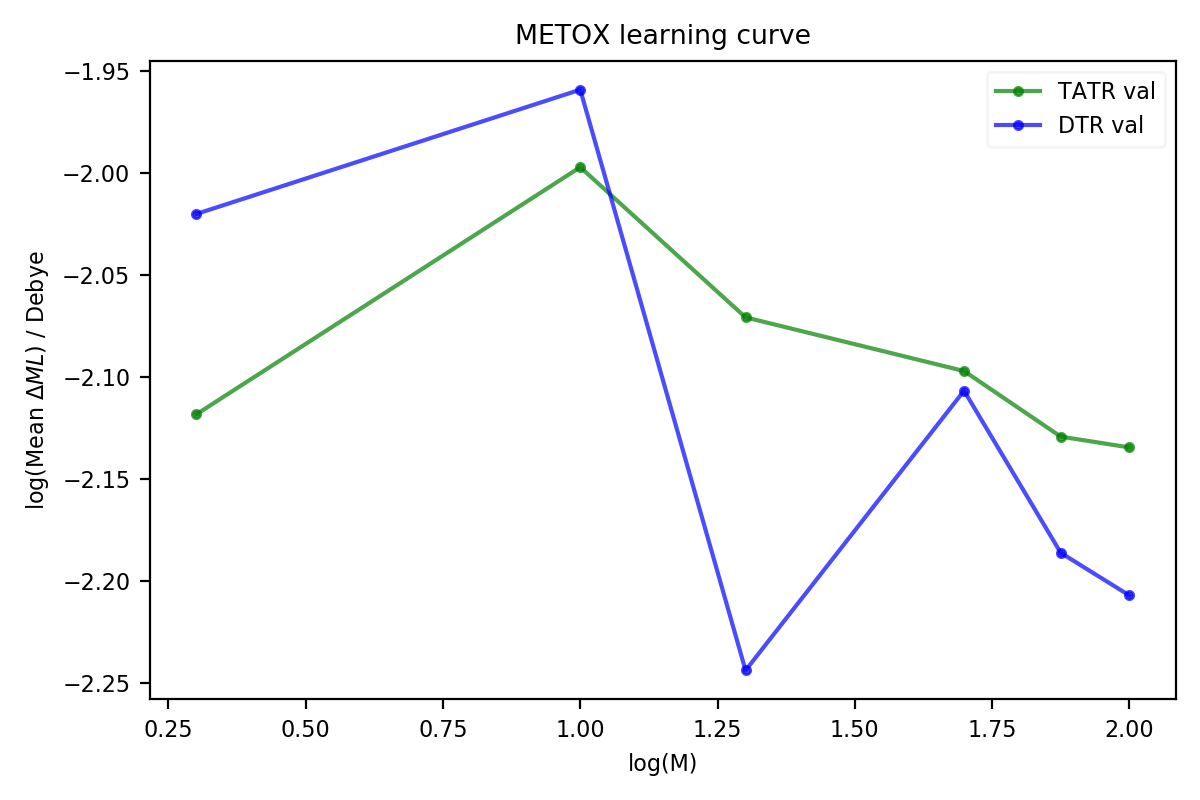
\includegraphics[scale=1.0]{p2/figures/si/METOX_learn_log_d.png}
    \caption{DTR and TATR validation curves for ($\textit{S}$)-methyloxirane correlated dipole.}
\end{figure}

\begin{figure}
    \centering
    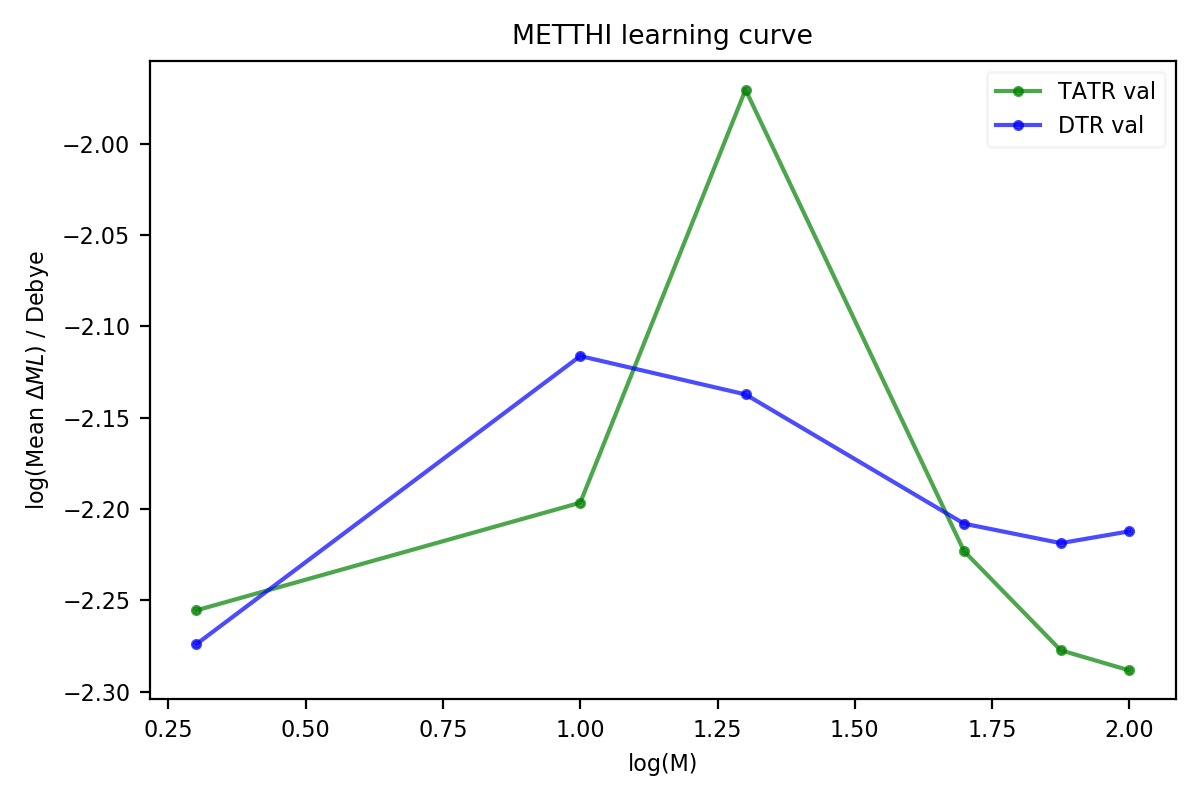
\includegraphics[scale=1.0]{p2/figures/si/METTHI_learn_log_d.png}
    \caption{DTR and TATR validation curves for ($\textit{R}$)-methylthiirane correlated dipole.}
\end{figure}
